\chapter{Pseudorandom functions from pseudorandom generators and CPA
security}\label{5-Pseudorandom-functions}

In this lecture we will see that the PRG conjecture implies the PRF
conjecture. We will also see how PRFs imply an encryption scheme that is
secure even when we encrypt multiple messages with the same key.

We have seen that PRF's (pseudorandom functions) are extremely useful,
and we'll see some more applications of them later on. But are they
perhaps too amazing to exist? Why would someone imagine that such a
wonderful object is feasible? The answer is the following theorem:

\hypertarget{prfthm}{}
\begin{theorem}[The PRF Theorem] \label[theorem]{prfthm}

Suppose that the PRG Conjecture is true, then there exists a secure PRF
collection \(\{ f_s \}_{s\in\{0,1\}^*}\) such that for every
\(s\in\{0,1\}^n\), \(f_s\) maps \(\{0,1\}^n\) to \(\{0,1\}^n\).

\end{theorem}

\begin{figure}
\centering
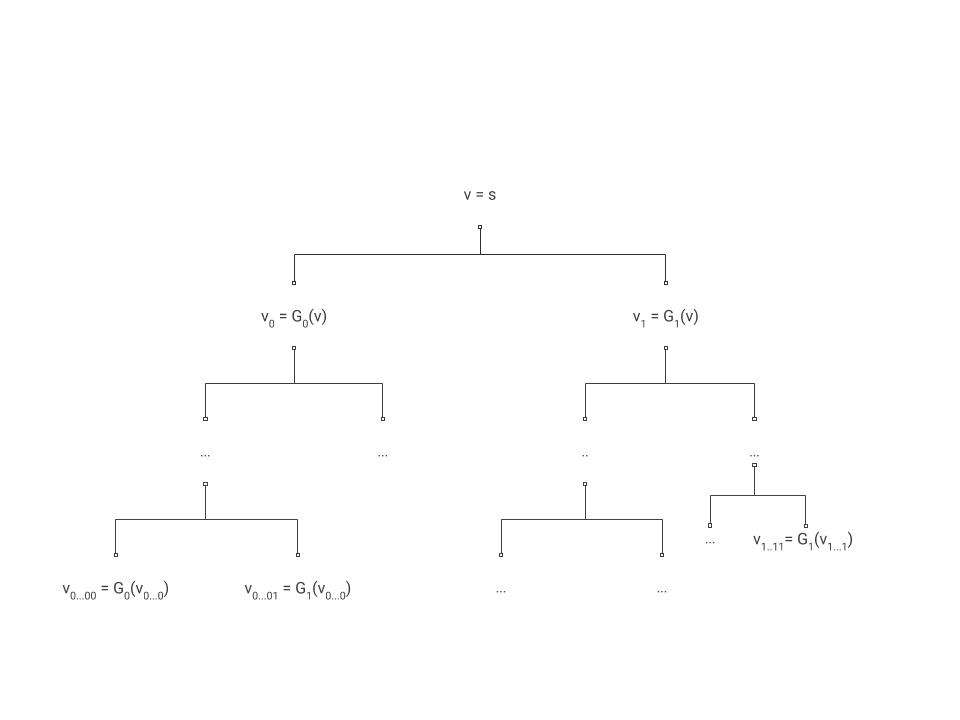
\includegraphics[width=\textwidth, height=0.25\paperheight, keepaspectratio]{../figure/PRF_from_PRG.jpg}
\caption{The construction of a pseudorandom function from a pseudorandom
generator can be illustrated by a depth \(n\) binary tree. The root is
labeled by the seed \(s\) and for every internal node \(v\) labeled by a
strong \(x\in\{0,1\}^n\), we use that label \(x\) as a seed into the PRG
\(G\) to label \(v\)'s two children. In particular, the children of
\(v\) are labeled with \(G_0(x)\) and \(G_1(x)\) respectively. The
output of the function \(f_s\) on input \(i\) is the label of the
\(i^{th}\) leaf counting from left to right. Note that the numbering of
leaf \(i\) is related to the bitstring representation of \(i\) and the
path leaf \(i\) in the following way: we traverse to leaf \(i\) from the
root by reading off the \(n\) bits of \(i\) left to right and descend
into the left child of the current node for every 0 we encounter and
traverse right for every 1.}
\label{PRFfromPRGfig}
\end{figure}

\begin{proof} \label[proof]{5-We-describe-the-proof-}

We describe the proof, see also
\href{https://web.engr.oregonstate.edu/~rosulekm/crypto/chap6.pdf}{Chapter
6 of Rosulek} or Section 8.5 of Katz-Lindell (section 7.5 in 2nd
edition) for alternative expositions.

If the PRG Conjecture is true then in particular by the length extension
theorem there exists a PRG \(G:\{0,1\}^n\rightarrow\{0,1\}^{2n}\) that
maps \(n\) bits into \(2n\) bits. Let's denote
\(G(s)=G_0(s)\circ G_1(s)\) where \(\circ\) denotes concatenation. That
is, \(G_0(s)\) denotes the first \(n\) bits and \(G_1(s)\) denotes the
last \(n\) bits of \(G(s)\).

For \(i\in\{0,1\}^n\), we define \(f_s(i)\) as
\begin{equation*}
G_{i_n}(G_{i_{n-1}}(\cdots G_{i_1}(s))).
\end{equation*}
This corresponds to \(n\) composed applications of \(G_{b}\) for
\(b \in \{0,1\}\). If the \(j^{th}\) bit of \(i\)'s binary string is 0
then the \(j^{th}\) application of the PRG is \(G_{0}\) otherwise it is
\(G_{1}\). This series of successive applications starts with the
initial seed \(s\).

This definition directly corresponds to the depiction in
\cref{PRFfromPRGfig}, where the successive applications of \(G_{b}\)
correspond to the recursive labeling procedure.

By the definition above we can see that to evaluate \(f_s(i)\) we need
to evaluate the pseudorandom generator \(n\) times on inputs of length
\(n\), and so if the pseudorandom generator is efficiently computable
then so is the pseudorandom function. Thus, ``all'' that's left is to
prove that the construction is secure and this is the heart of this
proof.

I've mentioned before that the first step of writing a proof is
convincing yourself that the statement is true, but there is actually an
often more important zeroth step which is understanding what the
statement actually \emph{means}. In this case what we need to prove is
the following:

We need to show that the security of the PRG \(G\) implies the security
of the PRF ensemble \(\{ f_s \}\). Via the contrapositive, this means
that we assume that there is an adversary \(A\) that can distinguish in
time \(T\) a black box for \(f_s(\cdot)\) from a black-box for a random
function with advantage \(\epsilon\). We need to use \(A\) come up with
an adversary \(D\) that can distinguish in time \(poly(T)\) an input of
the form \(G(s)\) (where \(s\) is random in \(\{0,1\}^n\)) from an input
of the form \(y\) where \(y\) is random in \(\{0,1\}^{2n}\) with bias at
least \(\epsilon/poly(T)\).

\begin{marginfigure}
\centering
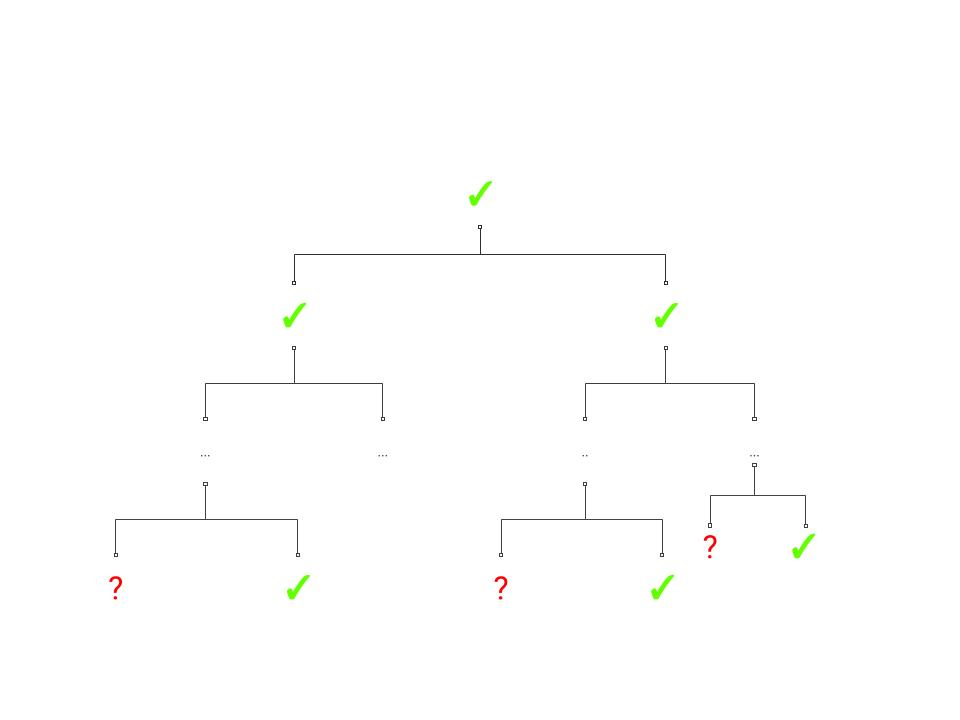
\includegraphics[width=\linewidth, height=1.5in, keepaspectratio]{../figure/Lazy_PRF_from_PRG.jpg}
\caption{In the ``lazy evaluation'' implementation of the black box to
the adversary, we label every node in the tree only when we need it.
Subsequent traversals do not reevaluate the PRG, leading to reuse of the
intermediate seeds. Thus for example, two sibling leaves will correspond
to a single call to \(G(x)\), where \(x\) is their parent's label, but
with the left child receiving the first \(n\) bits and the right child
receiving the second \(n\) bits of \(G(x)\). In this figure check marks
correspond to nodes that have been labeled and question marks to nodes
that are still unlabeled.}
\label{lazyevalprffig}
\end{marginfigure}

Assume that \(A\) as above is a \(T\)-time adversary that wins in the
``PRF game'' with advantage \(\epsilon\). Let us consider the ``lazy
evaluation'' implementation of the black box for \(A\) illustrated in
\cref{lazyevalprffig}. That is, at every point in time there are nodes
in the full binary tree that are labeled and nodes which we haven't yet
labeled. When \(A\) makes a query \(i\), this query corresponds to the
path \(i_1\ldots i_n\) in the tree. We look at the lowest (furthest away
from the root) node \(v\) on this path which has been labeled by some
value \(y\), and then we continue labelling the path from \(v\)
downwards until we reach \(i\). In other words, we label the two
children of \(v\) by \(G_0(y)\) and \(G_1(y)\), and then if the path
\(i\) involves the first child then we label its children by
\(G_0(G_0(y))\) and \(G_1(G_0(y))\), and so on and so forth (see
\cref{oracleevaltreefig}). Note that because \(G_{0}(y)\) and
\(G_{1}(y)\) correspond to a single call to \(G\), regardless of whether
the traversals continues left or right (i.e.~whether the current level
corresponds to a value 0 or 1 in \(i\)) we label both children at the
same time.

\begin{figure}
\centering
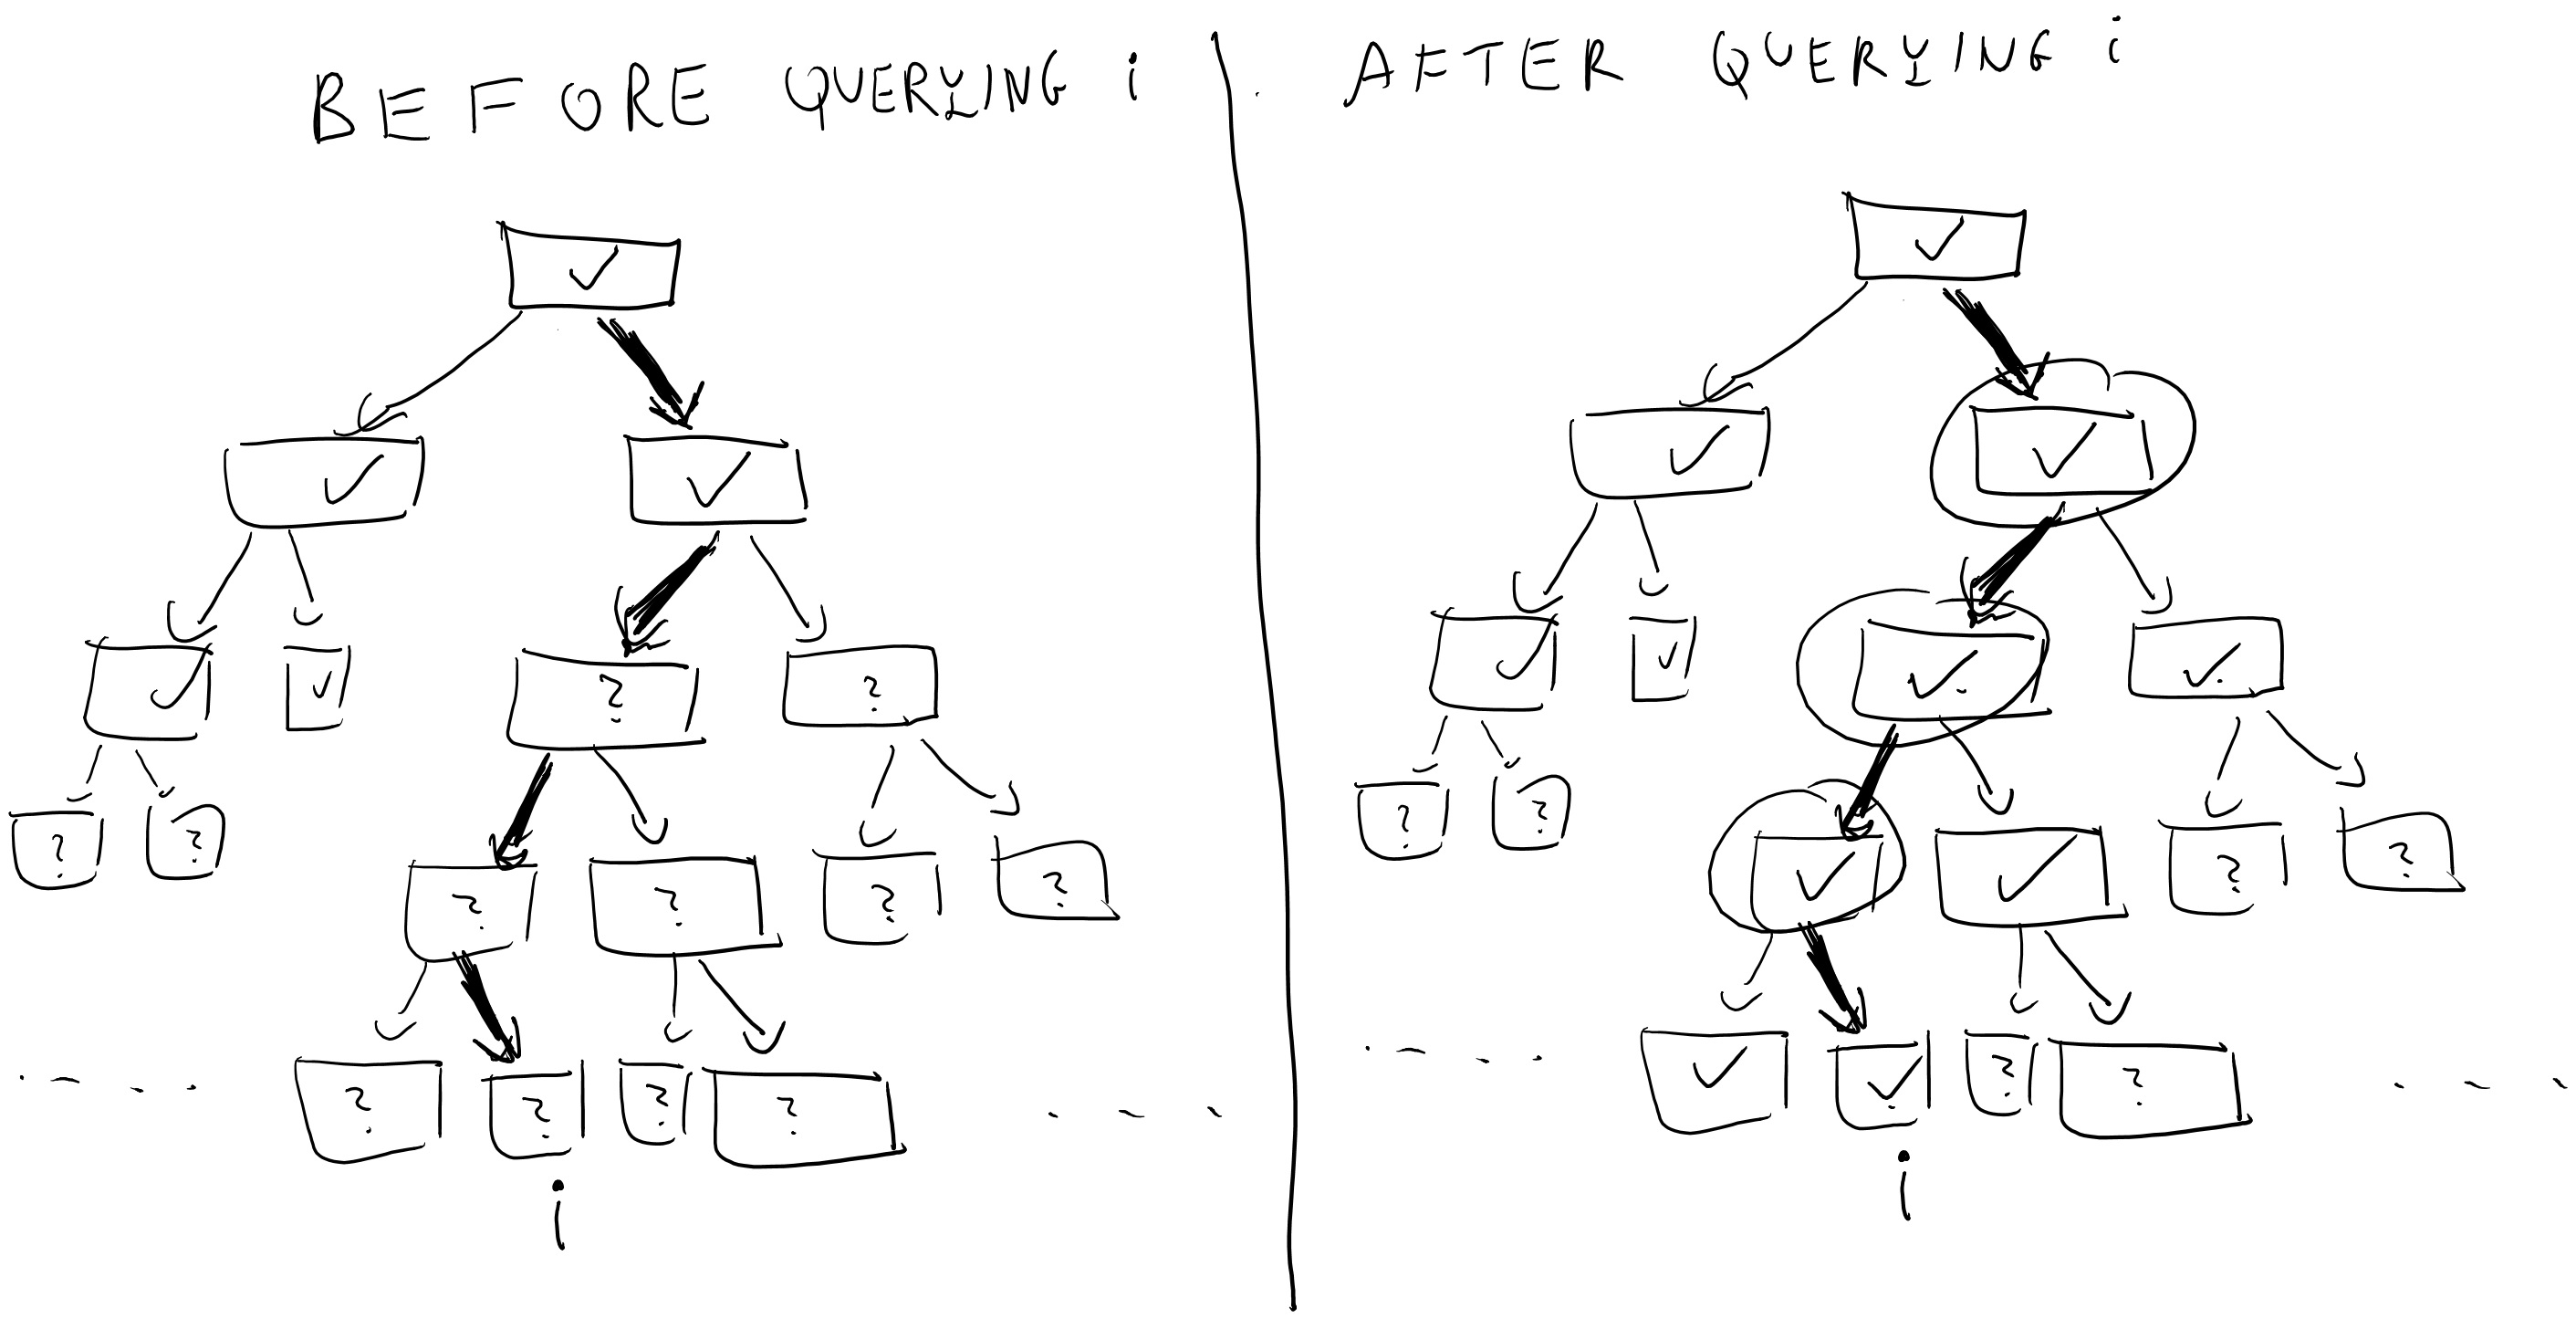
\includegraphics[width=\textwidth, height=0.25\paperheight, keepaspectratio]{../figure/prf-oracle-step.jpg}
\caption{When the adversary queries \(i\), the oracle takes the path
from \(i\) to the root and computes the generator on the minimum number
of internal nodes that is needed to obtain the label of the \(i^{th}\)
leaf.}
\label{oracleevaltreefig}
\end{figure}

A moment's thought shows that this is just another (arguably cumbersome)
way to describe the oracle that simply computes the map
\(i\mapsto f_s(i)\). And so the experiment of running \(A\) with this
oracle produces precisely the same result as running \(A\) with access
to \(f_s(\cdot)\). Note that since \(A\) has running time at most \(T\),
the number of times our oracle will need to label an internal node is at
most \(T' \leq 2nT\) (since we label at most \(2n\) nodes for every
query \(i\)).

We now define the following \(T'\) hybrids: in the \(j^{th}\) hybrid, we
run this experiment but in the first \(j\) times the oracle needs to
label internal nodes then it uses independent random labels. That is,
for the first \(j\) times we label a node \(v\), instead of letting the
label of \(v\) be \(G_b(u)\) (where \(u\) is the parent of \(v\), and
\(b\in \{0,1\}\) corresponds to whether \(v\) is the left or right child
of \(u\)), we label \(v\) by a random string in \(\{0,1\}^n\).

\begin{figure}
\centering
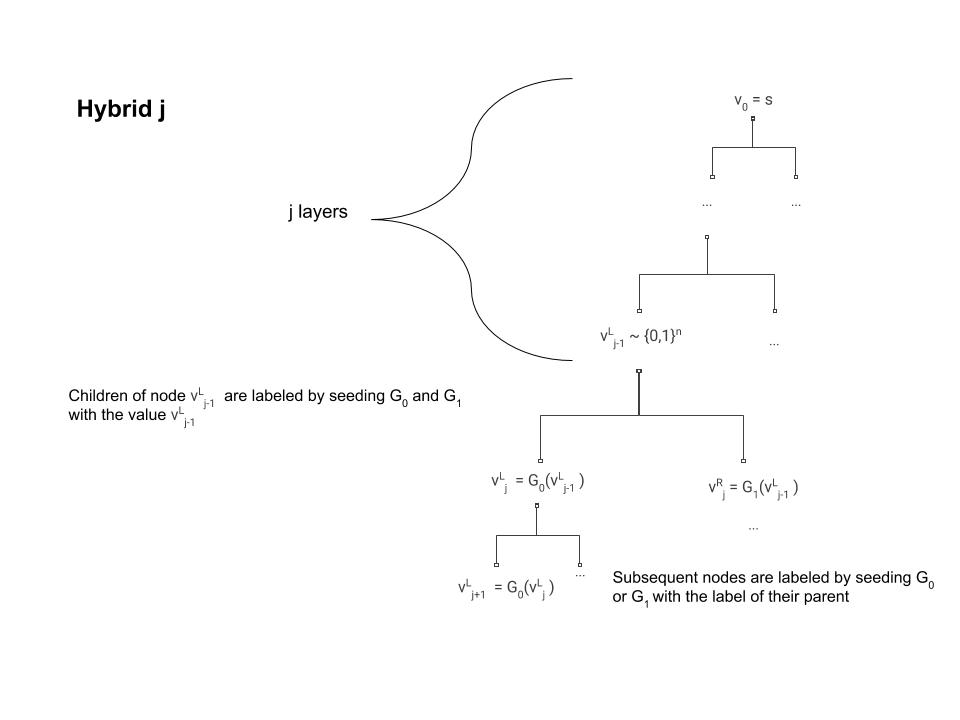
\includegraphics[width=\textwidth, height=0.25\paperheight, keepaspectratio]{../figure/hybrid_j_thm_5-1.jpg}
\caption{In the \(j^{th}\) hybrid the first \(j\) internal labels are
drawn uniformly at random from \(U_{n}\). All subsequent children's
labels are produced in the usual way by seeding \(G\) with the label
\(z\) of the parent and assigning the first \(n\) bits (\(G_{0}(z)\)) to
the left child and the last \(n\) bits (\(G_{1}(z)\)) to the right
child. For example, for some node \(v^{L}_{j-1}\) at the \(j^{th}\)
level, we generate pseudorandom string \(G(v^{L}_{j-1})\) and label the
left child \(v^{L}_{j} = G_{0}(v^{L}_{j-1})\) and the right child
\(v^{R}_{j} = G_{1}(v^{L}_{j-1})\). Note that the labeling scheme for
this diagram is different from that in the previous figures. This is
simply for ease of exposition, we could still index our nodes via the
path reaching them from the root.}
\label{hybridj}
\end{figure}

\begin{figure}
\centering
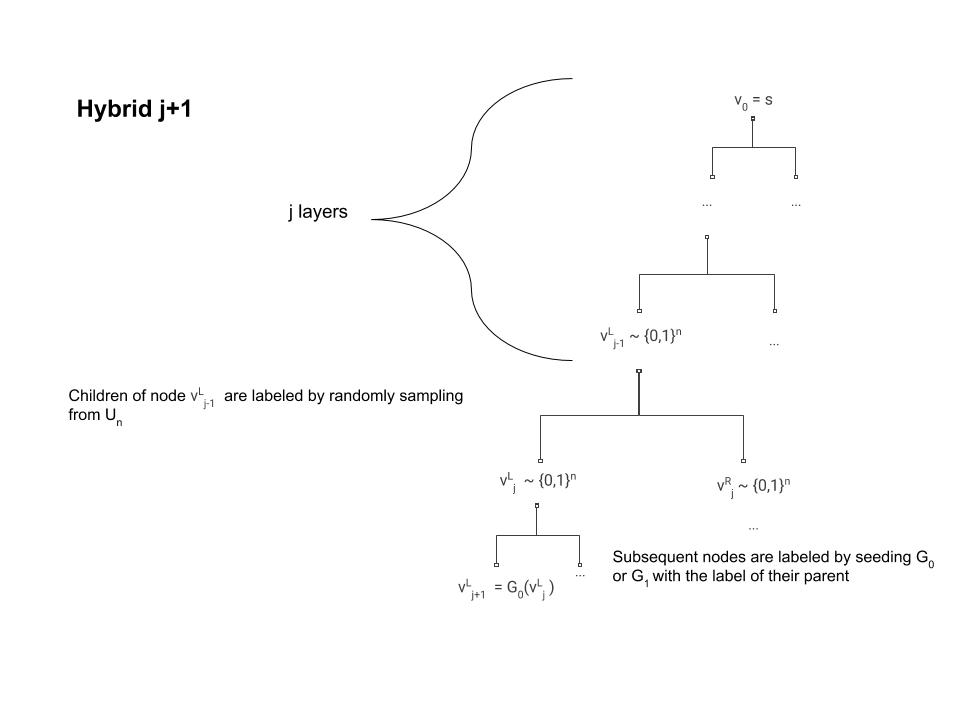
\includegraphics[width=\textwidth, height=0.25\paperheight, keepaspectratio]{../figure/hybrid_j1_thm_5-1.jpg}
\caption{The \(j+1^{st}\) hybrid differs from the \(j^{th}\) in that the
process of assigning random labels continues until the \(j+1^{st}\) step
as opposed to the \(j^{th}\). The hybrids are otherwise completely
identically constructed.}
\label{hybridj1}
\end{figure}

Note that the \(0^{th}\) hybrid corresponds to the case where the oracle
implements the function \(i\mapsto f_s(i)\), while in the \(T'^{th}\)
hybrid all labels are random and hence implements a random function. By
the hybrid argument, if \(A\) can distinguish between the \(0^{th}\)
hybrid and the \(T'^{th}\) hybrid with bias \(\epsilon\) then there must
exists some \(j\) such that it distinguishes between the \(j^{th}\)
hybrid (pictured in \cref{hybridj}) and the \(j+1^{st}\) hybrid
(pictured in \cref{hybridj1}) with bias at least \(\epsilon/T'\). We
will use this \(j\) and \(A\) to break the pseudorandom generator.

\begin{figure}
\centering
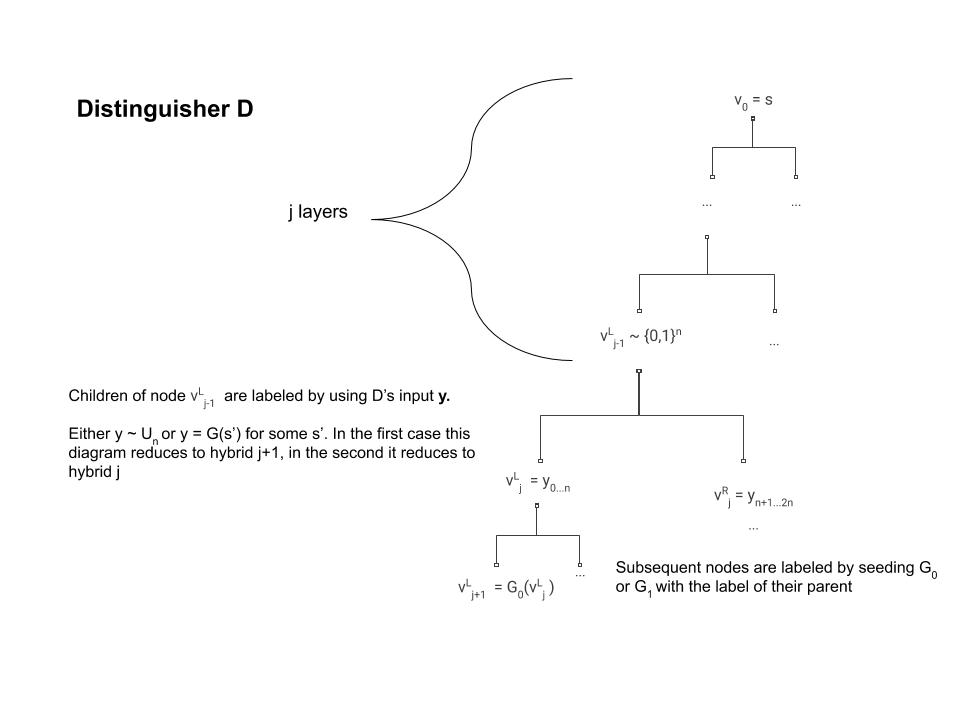
\includegraphics[width=\textwidth, height=0.25\paperheight, keepaspectratio]{../figure/distinguisher_D_thm_5-1.jpg}
\caption{Distinguisher D is similar to hybrid \(j\), in that the nodes
in the first \(j\) layers are assigned completely random labels. When
evaluating along a particular path through \(v_{j-1}^{L}\), rather than
labeling the two children by applying \(G\) to its label, it simply
splits the input \(y\) into two strings \(y_{0...n}\),\(y_{n+1...2n}\).
If \(y\) is truly random, \(D\) is identical to hybrid \(j+1\). If
\(y=G(s)\) for some random seed \(s\), then \(D\) simulates hybrid
\(j\).}
\label{distinguisherd}
\end{figure}

We can now describe our distinguisher \(D\) (see \cref{distinguisherd})
for the pseudorandom generator. On input a string \(y\in\{0,1\}^{2n}\)
\(D\) will run \(A\) and the \(j^{th}\) oracle inside its belly with one
difference- when the time comes to label the \(j^{th}\) node, instead of
doing this by applying the pseudorandom generator to the label of its
parent \(v\) (which is what should happen in the \(j^{th}\) oracle) it
uses its input \(y\) to label the two children of \(v\).

Now, if \(y\) was completely random then we get exactly the distribution
of the \(j+1^{st}\) oracle, and hence in this case \(D\) simulates
internally the \(j+1^{st}\) hybrid. However, if \(y=G(s)\) for some
randomly sampled \(s\in\{0,1\}^n\), though it may not be obvious at
first, we actually get the distribution of the \(j^{th}\) oracle.

The equivalence between hybrid \(j\) and distinguisher \(D\) under the
condition that \(y=G(s)\) is non obvious, because in hybrid \(j\), the
label for the children of \(v_{j-1}^{L}\) was supposed to be the result
of applying the pseudorandom generator to the label of \(v_{j-1}^{L}\)
and not to some other random string (see \cref{distinguisherd}).
However, because \(v\) was labeled \emph{before} the \(j^{th}\) step
then we know that it was actually labeled by a random string. Moreover,
since we use lazy evaluation we know that step \(j\) is the \emph{first}
time where we actually use the value of the label of \(v\). Hence, if at
this point we \emph{resampled} this label and used a completely
independent random string \(s\) then the distribution of \(v_{j-1}^{L}\)
and \(s\) would be \emph{identical}.

The key observations here are:

\begin{enumerate}
\def\labelenumi{\arabic{enumi}.}
\item
  The output of \(A\) does not directly depend on the internal labels,
  but only on the labels of the leaves (since those are the only values
  returned by the oracle).
\item
  The label for an internal vertex \(v\) is only used once, and that is
  for generating the labels for its children.
\end{enumerate}

Hence the distribution of \(y=G(s)\), for \(s\) drawn from \(U_n\), is
identical to the distribution, \(G(v_{j-1}^{L})\), of the \(j^{th}\)
hybrid, and thus if \(A\) had advantage \(\epsilon\) in breaking the PRF
\(\{ f_s \}\) then \(D\) will have advantage \(\epsilon/T'\) in breaking
the PRG \(G\) thus obtaining a contradiction.

\end{proof}

\hypertarget{prfpracticerem}{}
\begin{remark}[PRF's in practice] \label[remark]{prfpracticerem}

While this construction reassures us that we can rely on the existence
of pseudorandom functions even on days where we remember to take our
meds, this is not the construction people use when they need a PRF in
practice because it is still somewhat inefficient, making \(n\) calls to
the underlying pseudorandom generators. There are constructions (e.g.,
HMAC) based on hash functions that require stronger assumptions but can
use as few as two calls to the underlying function. We will cover these
constructions when we talk about hash functions and the random oracle
model. One can also obtain practical constructions of PRFs from
\emph{block ciphers}, which we'll see later in this lecture.

\end{remark}

\section{Securely encrypting many messages - chosen plaintext
security}\label{5-Securely-encrypting-ma}

Let's get back to our favorite task of \emph{encryption}. We seemed to
have nailed down the definition of secure encryption, or did we?

\begin{pause} \label[pause]{5-Try-to-think-what-kind}

Try to think what kind of security guarantees are \emph{not} provided by
the notion of computational secrecy we saw in \cref{compsecdef}

\end{pause}

\cref{compsecdef} talks about encrypting a \emph{single} message, but
this is not how we use encryption in the real world. Typically, Alice
and Bob (or Amazon and Boaz) setup a shared key and then engage in many
back and forth messages between one another. At first, we might think
that this issue of a single long message vs.~many short ones is merely a
technicality. After all, if Alice wants to send a sequence of messages
\((m_1,m_2,\ldots,m_t)\) to Bob, she can simply treat them as a single
long message. Moreover, the way that \emph{stream ciphers} work, Alice
can compute the encryption for the first few bits of the message she
decides what will be the next bits and so she can send the encryption of
\(m_1\) to Bob and later the encryption of \(m_2\). There is some truth
to this sentiment, but there are issues with using stream ciphers for
multiple messages. For Alice and Bob to encrypt messages in this way,
they must maintain a \emph{synchronized shared state}. If the message
\(m_1\) was dropped by the network, then Bob would not be able to
decrypt correctly the encryption of \(m_2\).

There is another way in which treating many messages as a single tuple
is unsatisfactory. In real life, Eve might be able to have some impact
on \emph{what} messages Alice encrypts. For example, the Katz-Lindell
book describes several instances in World War II where Allied forces
made particular military maneuver for the sole purpose of causing the
axis forces to send encryptions of messages of the Allies' choosing. To
consider a more modern example, today Google uses encryption for all of
its search traffic including (for the most part) the \emph{ads} that are
displayed on the page. But this means that an attacker, by paying
Google, can cause it to encrypt arbitrary text of their choosing. This
kind of attack, where Eve \emph{chooses} the message she wants to be
encrypted is called a \emph{chosen plaintext attack}. You might think
that we are already covering this with our current definition that
requires security \emph{for every} pair of messages and so in particular
this pair could chosen by Eve. However, in the case of multiple
messages, we would want to allow Eve to be able to choose \(m_2\)
\emph{after} she saw the encryption of \(m_1\).

All that leads us to the following definition, which is a strengthening
of our definition of computational security:

\hypertarget{cpasecuredef}{}
\begin{definition}[Chosen Plaintext Attack (CPA) secure encryption] \label[definition]{cpasecuredef}

An encryption scheme \((E,D)\) is \emph{secure against chosen plaintext
attack (CPA secure)} if for every polynomial time \(Eve\), Eve wins with
probability at most \(1/2+negl(n)\) in the game defined below:

\begin{enumerate}
\def\labelenumi{\arabic{enumi}.}
\tightlist
\item
  The key \(k\) is chosen at random in \(\{0,1\}^n\) and fixed.
\item
  Eve gets the length of the key \(1^n\) as input.\footnote{Giving Eve
    the key as a sequence of \(n\) \(1'\)s as opposed to in binary
    representation is a common notational convention in cryptography. It
    makes no difference except that it makes the input length for Eve of
    length \(n\), which makes sense since we want to allow Eve to run in
    \(poly(n)\) time.}
\item
  Eve interacts with \(E\) for \(t=poly(n)\) rounds as follows: in the
  \(i^{th}\) round, Eve chooses a message \(m_i\) and obtains
  \(c_i= E_k(m_i)\).
\item
  Then Eve chooses two messages \(m_0,m_1\), and gets \(c^* = E_k(m_b)\)
  for \(b\leftarrow_R\{0,1\}\).
\item
  Eve continues to interact with \(E\) for another \(poly(n)\) rounds,
  as in Step 3.
\item
  Eve \emph{wins} if she outputs \(b\).
\end{enumerate}

\end{definition}

\begin{marginfigure}
\centering
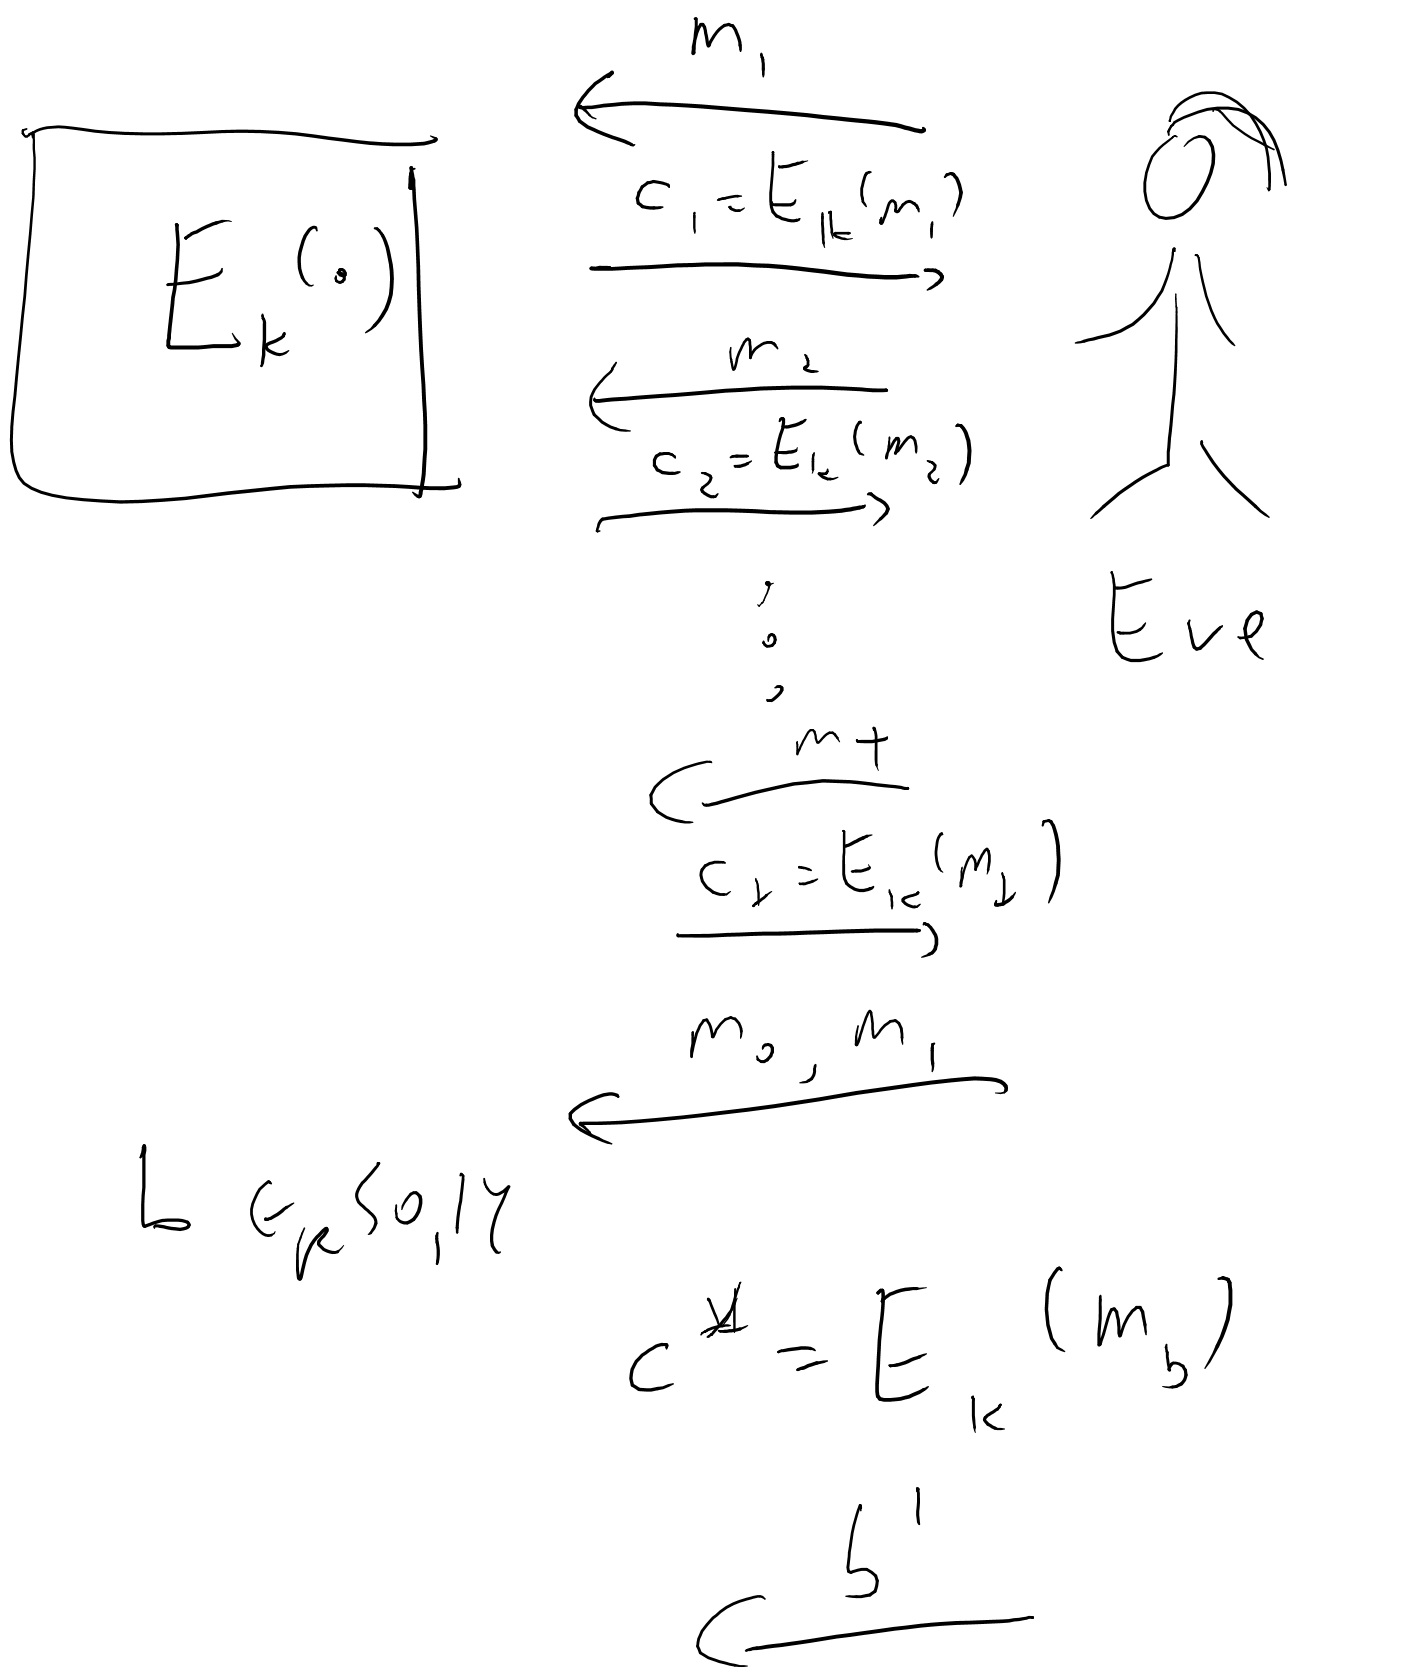
\includegraphics[width=\linewidth, height=1.5in, keepaspectratio]{../figure/cpa-game.jpg}
\caption{In the CPA game, Eve interacts with the encryption oracle and
at the end chooses \(m_0,m_1\), gets an encryption \(c^*=E_k(m_b)\) and
outputs \(b'\). She \emph{wins} if \(b'=b\)}
\label{cpasecgamefig}
\end{marginfigure}

\cref{cpasecuredef} is illustrated in \cref{cpasecgamefig}. Our previous
notion of computational secrecy (i.e., \cref{compsecdef}) corresponds to
the case that we skip Steps 3 and 5 above. Since Steps 3 and 5 only give
the adversary more power (and hence is only more likely to win), CPA
security (\cref{cpasecuredef}) is \emph{stronger} than computational
secrecy (\cref{compsecdef}), in the sense that every CPA secure
encryption \((E,D)\) is also computationally secure. It turns out that
CPA security is \emph{strictly stronger}, in the sense that without
modification, our stream ciphers cannot be CPA secure. In fact, we have
a stronger, and intially somewhat surprising theorem:

\hypertarget{CPAsecrandomthm}{}
\begin{theorem}[CPA security requires randomization] \label[theorem]{CPAsecrandomthm}

There is no CPA secure \((E,D)\) where \(E\) is \emph{deterministic}.

\end{theorem}

\begin{proof} \label[proof]{5-The-proof-is-very-simp}

The proof is very simple: Eve will only use a single round of
interacting with \(E\) where she will ask for the encryption \(c_1\) of
\(0^\ell\). In the second round, Eve will choose \(m_0=0^{\ell}\) and
\(m_1=1^{\ell}\), and get \(c^*=E_k(m_b)\) she wil then output \(0\) if
and only if \(c^*=c_1\).

\end{proof}

\begin{marginfigure}
\centering
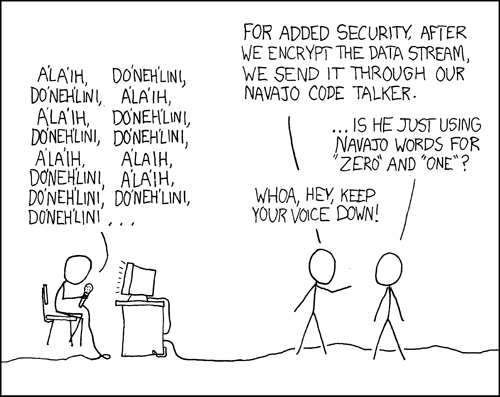
\includegraphics[width=\linewidth, height=1.5in, keepaspectratio]{../figure/code_talkers.png}
\caption{Insecurity of deterministic encryption}
\label{xkcdnavajotwofig}
\end{marginfigure}

This proof is so simple that you might think it shows a problem with the
definition, but it is actually a real problem with security. If you
encrypt many messages and some of them repeat themselves, it is possible
to get significant information by seeing the repetition pattern (que the
XKCD cartoon again, see \cref{xkcdnavajotwofig}). To avoid this issue we
need to use a \emph{randomized} (or \emph{probabilistic}) encryption,
such that if we encrypt the same message twice we \emph{won't} see two
copies of the same ciphertext.\footnote{If the messages are guaranteed
  to have \emph{high entropy} which roughly means that the probability
  that a message repeats itself is negligible, then it is possible to
  have a secure deterministic private-key encryption, and this is
  sometimes used in practice. (Though often some sort of randomization
  or padding is added to ensure this property, hence in effect creating
  a randomized encryption.) Deterministic encryptions can sometimes be
  useful for applications such as efficient queries on encrypted
  databases. See \href{https://goo.gl/GWJLFd}{this lecture} in Dan
  Boneh's coursera course.} But how do we do that? Here pseudorandom
functions come to the rescue:

\hypertarget{cpafromprfthm}{}
\begin{theorem}[CPA security from PRFs] \label[theorem]{cpafromprfthm}

Suppose that \(\{ f_s \}\) is a PRF collection where
\(f_s:\{0,1\}^n\rightarrow\{0,1\}^\ell\), then the following is a CPA
secure encryption scheme: \(E_s(m)=(r,f_s(r)\oplus m)\) where
\(r \leftarrow_R \{0,1\}^n\), and \(D_s(r,z)=f_s(r)\oplus z\).

\end{theorem}

\begin{proof} \label[proof]{5-I-leave-to-you-to-veri}

I leave to you to verify that \(D_s(E_s(m))=m\). We need to show the CPA
security property. As is usual in PRF-based constructions, we first show
that this scheme will be secure if \(f_s\) was an actually random
function, and then use that to derive security.

Consider the game above when played with a completely random function
and let \(r_i\) be the random string chosen by \(E\) in the \(i^{th}\)
round and \(r^*\) the string chosen in the last round. We start with the
following simple but crucial claim:

\textbf{Claim:} The probability that \(r^*=r_i\) for some \(i\) is at
most \(T/2^n\).

\textbf{Proof of claim:} For any particular \(i\), since \(r^*\) is
chosen independently of \(r_i\), the probability that \(r^*=r_i\) is
\(2^{-n}\). Hence the claim follows from the union bound. QED

Given this claim we know that with probability \(1-T/2^n\) (which is
\(1-negl(n)\)), the string \(r^*\) is distinct from any string that was
chosen before. This means that by the lazy evaluation principle, if
\(f_s(\cdot)\) is a completely random function then the value
\(f_s(r^*)\) can be thought of as being chosen at random in the final
round independently of anything that happened before. But then
\(f_s(r^*)\oplus m_b\) amounts to simply using the one-time pad to
encrypt \(m_b\). That is, the distributions \(f_s(r^*)\oplus m_0\) and
\(f_s(r^*)\oplus m_1\) (where we think of \(r^*,m_0,m_1\) as fixed and
the randomness comes from the choice of the random function
\(f_s(\cdot)\)) are both equal to the uniform distribution \(U_n\) over
\(\{0,1\}^n\) and hence Eve gets absolutely no information about \(b\).

This shows that if \(f_s(\cdot)\) was a random function then Eve would
win the game with probability at most \(1/2\). Now if we have some
efficient Eve that wins the game with probability at least
\(1/2+\epsilon\) then we can build an adversary \(A\) for the PRF that
will run this entire game with black box access to \(f_s(\cdot)\) and
will output \(1\) if and only if Eve wins. By the argument above, there
would be a difference of at least \(\epsilon\) in the probability it
outputs \(1\) when \(f_s(\cdot)\) is random vs when it is pseudorandom,
hence contradicting the security property of the PRF.

\end{proof}

\section{Pseudorandom permutations / block
ciphers}\label{5-Pseudorandom-permutati}

Now that we have pseudorandom functions, we might get greedy and want
such functions with even more magical properties. This is where the
notion of \emph{pseudorandom permutations} comes in.

::: \{.definition title=``Pseudorandom permutations'' \#PRPdef\} Let
\(\ell:\N \rightarrow \N\) be some function that is polynomially bounded
(i.e., there are some \(0<c<C\) such that \(n^c < \ell(n) < n^C\) for
every \(n\)). A collection of functions \(\{ f_s \}\) where
\(f_s:\{0,1\}^{\ell} \rightarrow\{0,1\}^{\ell}\) for \(\ell=\ell(|s|)\)
is called a \emph{pseudorandom permutation (PRP) collection} if:

\begin{enumerate}
\def\labelenumi{\arabic{enumi}.}
\tightlist
\item
  It is a pseudorandom function collection (i.e., the map
  \(s,x \mapsto f_s(x)\) is efficiently computable and there is no
  efficient distinguisher between \(f_s(\cdot)\) with a random \(s\) and
  a random function).\\
\item
  Every function \(f_s\) is a permutation of \(\{0,1\}^\ell\) (i.e., a
  one to one and onto map).\\
\item
  There is an efficient algorithm that on input \(s,y\) returns
  \(f_s^{-1}(y)\). The parameter \(n\) is known as the \emph{key length}
  of the pseudorandom permutation collection and the parameter
  \(\ell=\ell(n)\) is known as the \emph{input length} or \emph{block
  length}. Often, \(\ell=n\) and so in most cases you can safely ignore
  this distinction.
\end{enumerate}

\begin{pause} \label[pause]{5-At-first-look-crefPRPd}

At first look \cref{PRPdef} might seem not to make sense, since on one
hand it requires the map \(x \mapsto f_s(x)\) to be a permutation, but
on the other hand it can be shown that with high probability a random
map \(H:\{0,1\}^\ell \rightarrow \{0,1\}^\ell\) will \emph{not} be a
permutation. How can then such a collection be pseudorandom? The key
insight is that while a random map might not be a permutation, it is not
possible to distinguish with a polynomial number of queries between a
black box that computes a random function and a black box that computes
a random permutation. Understanding why this is the case, and why this
means that \cref{PRPdef} is reasonable, is crucial to getting intuition
to this notion, and so I suggest you pause now and make sure you
understand these points.

\end{pause}

As usual with a new concept, we want to know whether it is possible to
achieve it and whether it is useful. The former is established by the
following theorem:

\hypertarget{PRPfromPRF}{}
\begin{theorem}[PRP's from PRFs] \label[theorem]{PRPfromPRF}

If the PRF conjecture holds (and hence by \cref{prfthm} also if the PRG
conjecture holds) then there exists a pseudorandom permutation
collection.

\end{theorem}

\begin{figure}
\centering
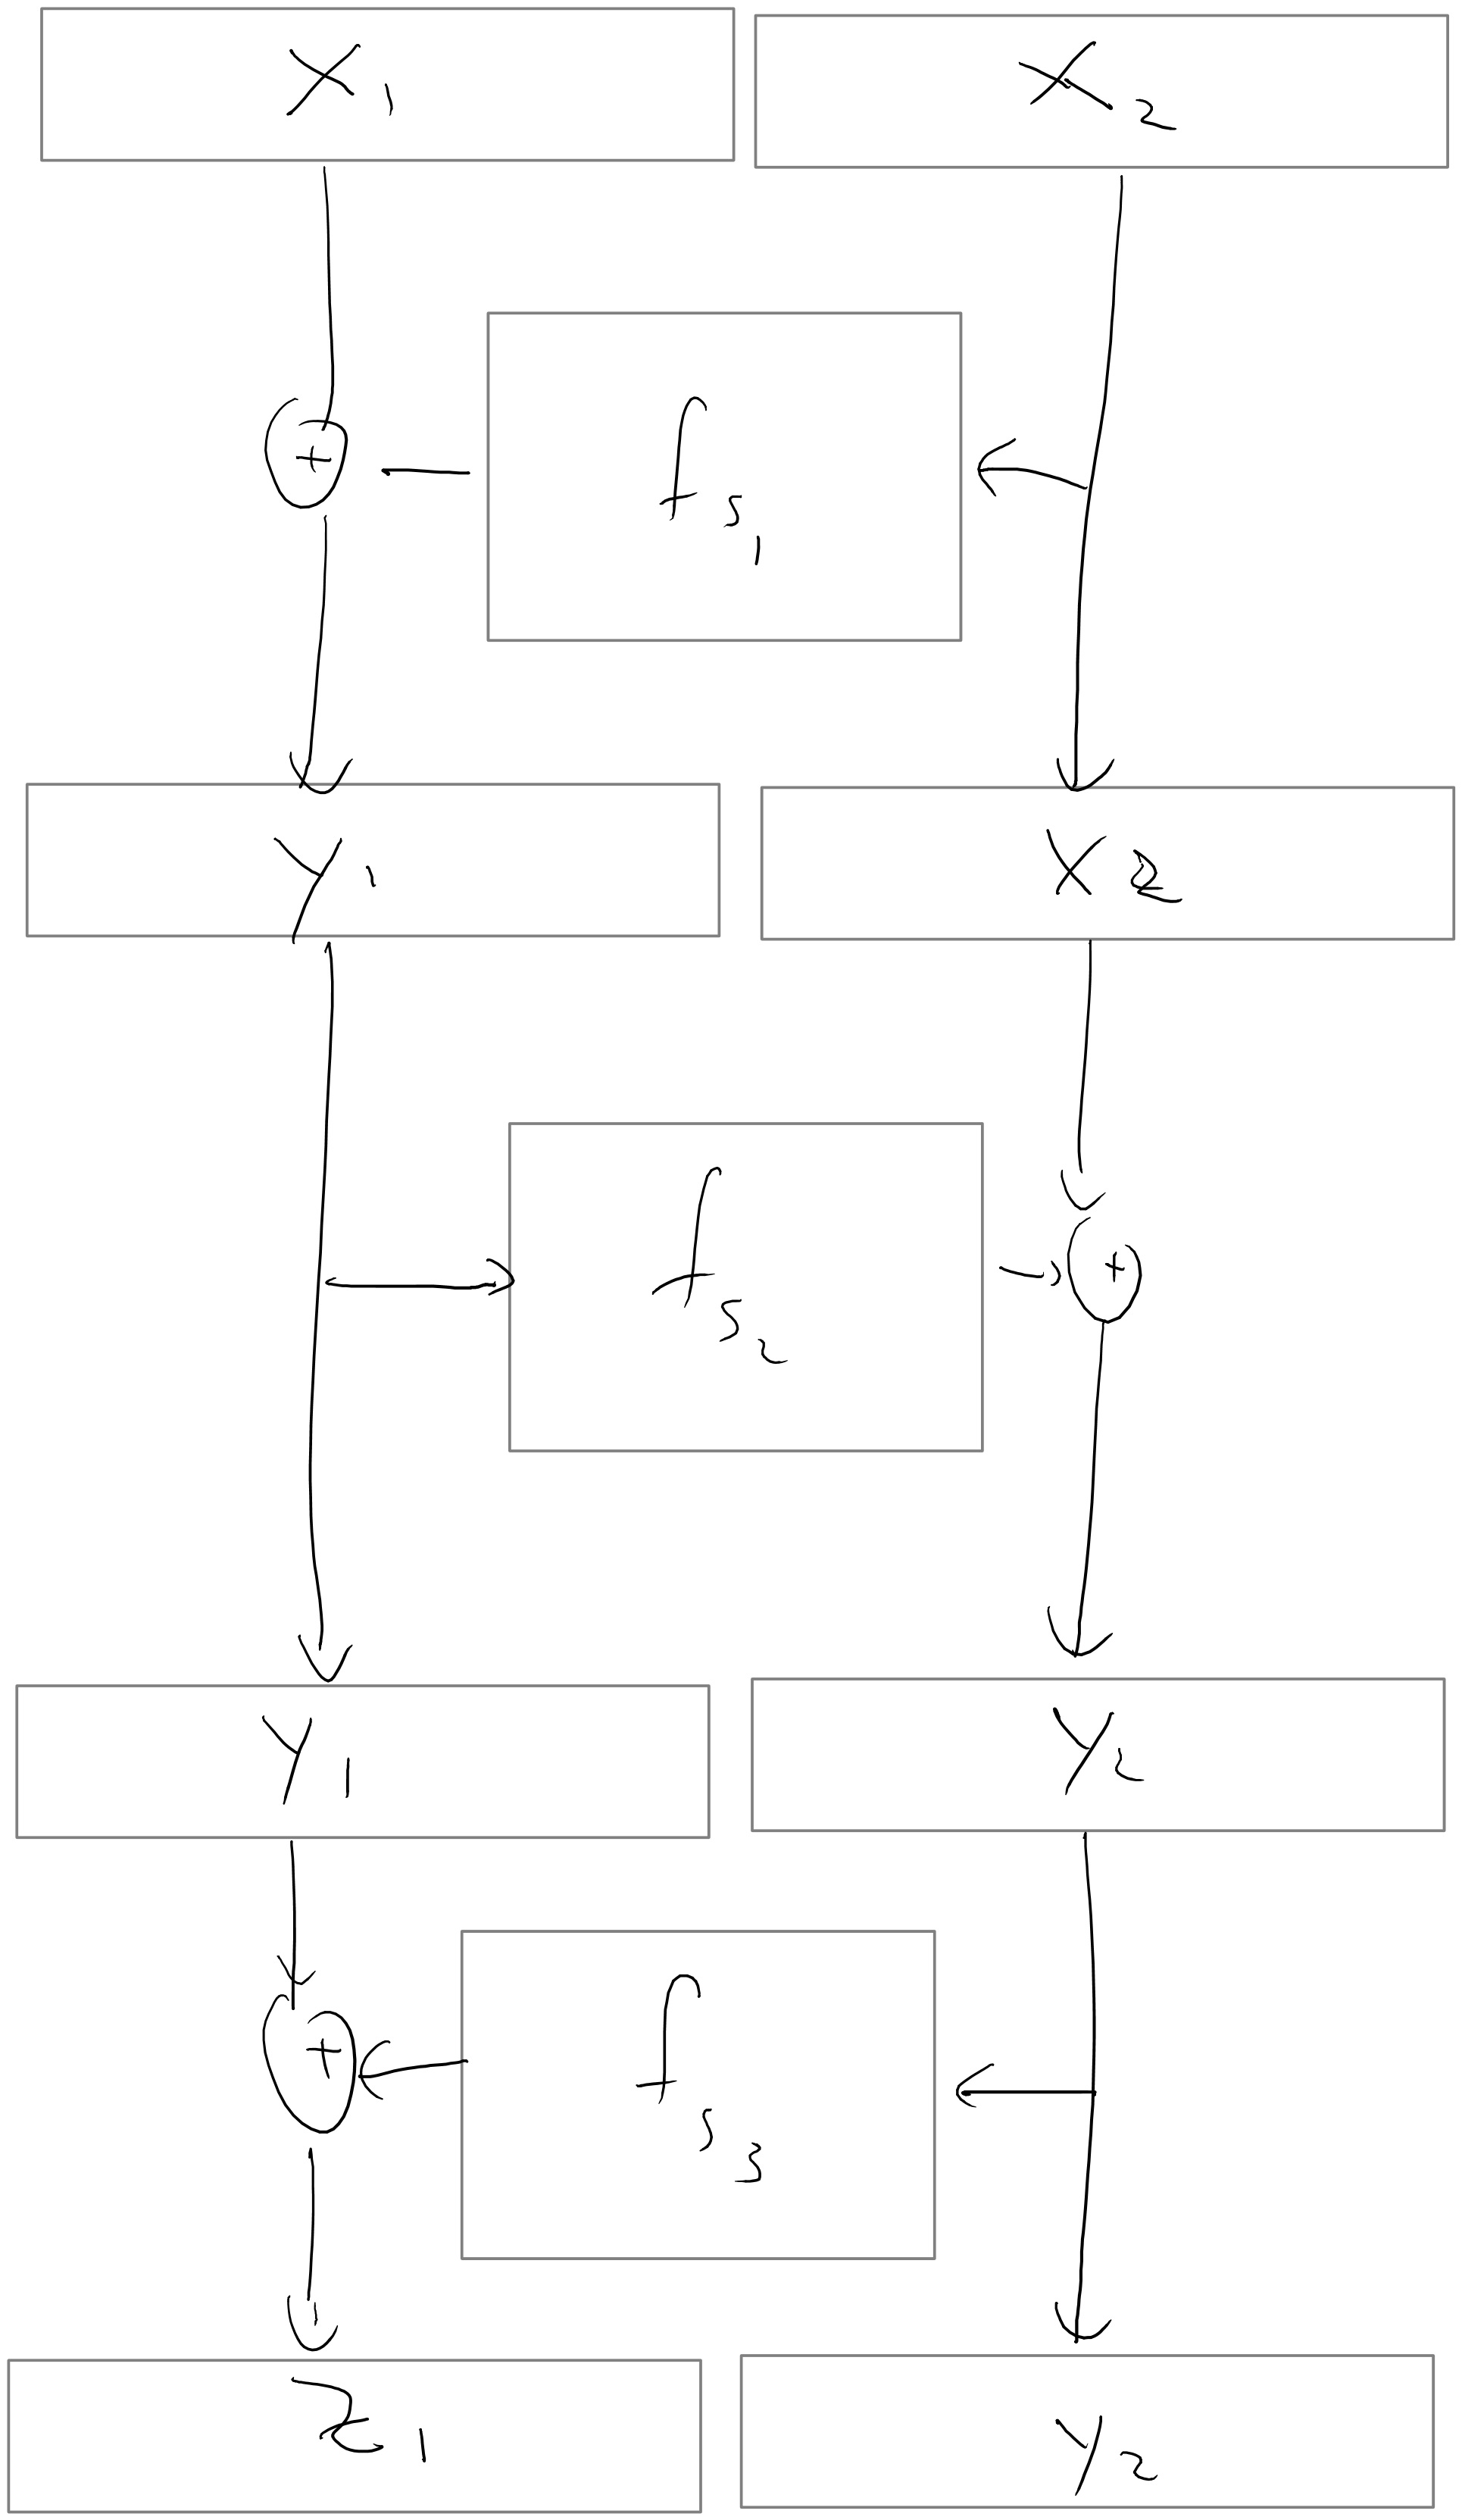
\includegraphics[width=\textwidth, height=0.25\paperheight, keepaspectratio]{../figure/feistel.jpg}
\caption{We build a PRP \(p\) on \(2n\) bits from three PRFs
\(f_{s_1},f_{s_2},f_{s_3}\) on \(n\) bits by letting
\(p_{s_1,s_2,s_3}(x_1,x_2)=(z_1,y_2)\) where
\(y_1 = x_1 \oplus f_{s_1}(x_2)\), \(y_2 = x_2 \oplus f_{s_2}(y_1)\) and
\(z_1 = f_{s_3}(y_2) \oplus y_1\).}
\label{feistelfig}
\end{figure}

\begin{proof} \label[proof]{5-creffeistelfig-illustr}

\cref{feistelfig} illustrates the construction of a pseudorandom
permutation from a pseudorandom function. The construction (known as the
Luby-Rackoff construction) uses several rounds of what is known as the
\href{https://en.wikipedia.org/wiki/Feistel_cipher}{Feistel
Transformation} that maps a function
\(f:\{0,1\}^n \rightarrow \{0,1\}^n\) into a permutation
\(g:\{0,1\}^{2n} \rightarrow \{0,1\}^{2n}\) using the map
\((x,y) \mapsto (x,f(x) \oplus y)\).

Specifically, given a PRF family \(\{f_s\}\) with \(n\)-bit keys,
inputs, and outputs, our candidate PRP family will be called
\(\{p_{s_1,s_2,s_3}\}\). Here,
\(p_{s_1,s_2, s_3}:\{0,1\}^{2n} \to \{0,1\}^{2n}\) is calculated on
input \((x_1, x_2) \in \{0,1\}^{2n}\) as follows (see
\cref{feistelfig}):

\begin{itemize}
\tightlist
\item
  First, map \((x_1, x_2) \mapsto (y_1, x_2)\), where
  \(y_1 = x_1 \oplus f_{s_1}(x_2)\).
\item
  Next, map \((y_1, x_2) \mapsto (y_1, y_2)\), where
  \(y_2 = x_2 \oplus f_{s_2}(y_1)\).
\item
  Next, map \((y_1, y_2) \mapsto (z_1, y_2)\), where
  \(z_1 = y_1 \oplus f_{s_3}(y_2)\).
\item
  Finally, output \(p_{s_1,s_2,s_3}(x_1,x_2) = (z_1, y_2)\).
\end{itemize}

Each of the first three steps above corresponds to a single round of the
Feistel transformation, which is easily seen to be both efficiently
computable \emph{and} efficiently invertible. In fact, we can
efficiently calculate \(p_{s_1,s_2,s_3}^{-1}(z_1, y_2)\) for an
arbitrary string \((z_1,y_2) \in \{0,1\}^{2n}\) by running the above
three rounds of Feistel transformations in reverse order.

Thus, the real challenge in proving \cref{PRPfromPRF} is not showing
that \(\{p_{s_1,s_2,s_3}\}\) is a valid permutation, but rather showing
that it is \emph{pseudorandom}. The details of remainder of this proof
are a bit technical, and can be safely skipped on a first reading.

Intuitively, the argument goes like this. Consider an oracle
\(\mathcal{O}\) for \(p_{s_1,s_2,s_3}\) that answers an adversary's
query \((x_1, x_2)\) by carrying out the three Feistel transformations
outlined above and outputting \((z_1, y_2)\). First, we'll show that
with high probability, \(\mathcal{O}\) will never encounter the same
intermediate string \(y_1\) twice, over the course of all queries
(unless the adversary makes a duplicate query). Since the string
\(y_1\), calculated in Step 1, determines the input on which \(f_{s_2}\)
is evaluated in Step 2, it follows that the strings \(y_2\) calculated
in Step 2 will appear to be chosen independently and at random. In
particular, \emph{they too} will be pairwise distinct with high
probability. Since the string \(y_2\) is in turn passed as input to
\(f_{s_3}\) in Step 3, it follows that the strings \(z_1\) encountered
over the course of all queries will also appear to be chosen
independently and at random. Ultimately, this means that the oracle's
outputs \((z_1, y_2)\) will look like freshly independent, random
strings.

To make this reasoning precise, notice first that it suffices to
establish the security of a \emph{variant} of \(p_{s_1,s_2,s_3}\) in
which the pseudorandom functions \(f_{s_1}\), \(f_{s_2}\), and
\(f_{s_3}\) used in the construction are replaced by truly random
functions \(h_1,h_2,h_3 : \{0,1\}^n \to \{0,1\}^n\). Call this variant
\(p_{h_1,h_2,h_3}\). Indeed, the assumption that \(\{f_s\}\) is a PRF
collection tells us that making this change has only a negligible effect
on the output of an adversary with oracle access to \(p\). With this in
mind, our job is to show that for every efficient adversary \(A\), the
difference
\(|\Pr[A^{p_{h_1,h_2,h_3}(\cdot)}(1^n)=1] - \Pr[A^{H(\cdot)}(1^n)=1]|\)
is negligible. In this expression, the first probability is taken over
the choice of the random functions
\(h_1,h_2,h_3 :\{0,1\}^n \to \{0,1\}^n\) used in the Feistel
transformation, and the second probability is taken over the random
function \(H : \{0,1\}^{2n} \to \{0,1\}^{2n}\). To simplify matters,
suppose without loss of generality that \(A\) always makes \(q(n)\)
\emph{distinct} queries to its oracle, denoted
\((x_1^{(1)}, x_2^{(1)}), \ldots, (x_1^{(q(n))}, x_2^{(q(n))})\) in
order. Similarly, let \(y_1^{(i)}, y_2^{(i)}, z_1^{(i)}\) denote the
intermediate strings calculated in the three rounds of the Feistel
transformation. Here, \(q\) is a polynomial in \(n\).

Consider the case in which the adversary \(A\) is interacting with the
oracle for \(p_{h_1,h_2,h_3}\), as opposed to the random oracle. Let us
say that a \emph{collision occurs at \(y_1\)} if for some
\(1 \le i < j \le q(n)\), the string \(y_1^{(i)}\) computed while
answering \(A\)'s \(i\)th query coincides with the string \(y_1^{(j)}\)
computed while answering \(A\)'s \(j\)th query. We claim the probability
that a collision occurs at \(y_1\) is negligibly small. Indeed, if a
collision occurs at \(y_1\), then \(y_1^{(i)} = y_1^{(j)}\) for some
\(i \neq j\). By the construction of \(p_{h_1,h_2,h_3}\), this means
that
\(x_1^{(i)} \oplus h_1(x_2^{(i)}) = x_1^{(j)} \oplus h_1(x_2^{(j)})\).
In particular, it cannot be the case that \(x_1^{(i)} \neq x_1^{(j)}\)
and \(x_2^{(i)} = x_2^{(j)}\). Since we assumed that \(A\) makes
distinct queries to its oracle, it follows that
\(x_2^{(i)} \neq x_2^{(j)}\) and hence that \(h_1(x_2^{(i)})\) and
\(h_1(x_2^{(j)})\) are uniform and independent. In other words,
\(\Pr[y_1^{(i)} = y_1^{(j)}] = \Pr[x_1^{(i)} \oplus f_1(x_2^{(i)}) = x_1^{(j)} \oplus f_1(x_2^{(j)})] = 2^{-n}\).
Taking a union bound over all choices of \(i\) and \(j\), we see that
the probability of a collision at \(y_1\) is at most \(q(n)^2/2^n\),
which is negligible.

Next, define a \emph{collision at \(y_2\)}, by a pair of queries
\(1 \le i < j \le q(n)\) such that \(y_2^{(i)} = y_2^{(j)}\). We argue
that the probability of a collision at \(y_2\) is also negligible,
provided that we condition on the overwhelmingly likely event that no
collision occurs at \(y_1\). Indeed, if \(y_1^{(i)} \neq y_1^{(j)}\) for
all \(i \neq j\), then \(h_2(y_1^{(1)}), \ldots, h_2(y_1^{(q(n))})\) are
distribued independently and uniformly at random. In particular, we have
\(\Pr[y_2^{(i)} = y_2^{(j)} \mid \text{no collision at }y_1] = 2^{-n}\),
which is negligible even after taking a union bound over all \(i\) and
\(j\). The same argument applied to the \emph{third} round of the
Feistel transformation similarly shows that, conditioned on the
overwhelmingly likely event that no collision occurs at \(y_1\) or
\(y_2\), the strings \(z_1^{(1)}, \ldots, z_1^{(i)}\) for
\(1 \le i \le q(n)\) are also distributed as fresh, independent, random
strings. At this point, we've shown that the adversary cannot
distinguish the outputs
\((z_1^{(1)}, y_2^{(1)}), \ldots, (z_1^{(q(n))}, y_2^{(q(n))})\) of the
oracle for \(p_{h_1,h_2,h_3}\) from the outputs of a random oracle
unless an event with negligibly small probability occurs. We conclude
that the collection \(\{p_{h_1,h_2,h_3}\}\), and hence our original
collection \(\{p_{s_1,s_2,s_3}\}\), is a secure PRP collection.

For more details regarding this proof, see Section 4.5 in Boneh Shoup or
Section 8.6 (7.6 in 2nd ed) in Katz-Lindell, whose proof was used as a
model for ours.

\end{proof}

\hypertarget{feistelrounds}{}
\begin{remark}[How many Feistel rounds?] \label[remark]{feistelrounds}

The construction in the proof of \cref{PRPfromPRF} constructed a PRP
\(p\) by performing \(3\) rounds of the Feistel transformation with a
known PRF \(f\). It is an interesting exercise to try to show that doing
just \(1\) or \(2\) rounds of the Feistel transformation \emph{does not}
suffice to achieve a PRP. \emph{Hint: consider an adversary that makes
queries of the form \((x_1, x_2)\) where \(x_2\) is held fixed and
\(x_1\) is varied.}

\end{remark}

The more common name for a pseudorandom permutation is \emph{block
cipher} (though typically block ciphers are expected to meet additional
security properties on top of being PRPs). The constructions for block
ciphers used in practice don't follow the construction of
\cref{PRPfromPRF} (though they use some of the ideas) but have a more
ad-hoc nature.

One of the first modern block ciphers was the
\href{https://goo.gl/XiCvjs}{Data Encryption Standard (DES)} constructed
by IBM in the 1970's. It is a fairly good cipher- to this day, as far as
we know, it provides a pretty good number of security bits compared to
its key length. The trouble is that its key is only \(56\) bits long,
which is no longer outside the reach of modern computing power. (It
turns out that subtle variants of DES are far less secure and fall prey
to a technique known as \href{https://goo.gl/GAvbh8}{differential
cryptanalysis}; the IBM designers of DES were aware of this technique
but kept it secret at the behest of the NSA.)

Between 1997 and 2001, the U.S. National Institute of Standards and
Technology (NIST) ran a competition to replace DES which resulted in the
adoption of the block cipher Rijndael as the new
\href{https://goo.gl/1HnqFb}{advanced encryption standard (AES)}. It has
a block size (i.e., input length) of 128 bits and a key size (i.e., seed
length) of 128, 196, or 256 bits.

The actual construction of AES (or DES for that matter) is not extremely
illuminating, but let us say a few words about the general principle
behind many block ciphers. They are typically constructed by repeating
one after the other a number of very simple permutations (see
\cref{blockcipherfig}). Each such iteration is called a \emph{round}. If
there are \(t\) rounds, then the key \(k\) is typically expanded into a
longer string, which we think of as a \(t\) tuple of strings
\((k_1,\ldots,k_t)\) via some pseudorandom generator known as the
\emph{key scheduling algorithm}. The \(i\)-th string in the tuple is
known as the \emph{round key} and is used in the \(i^{th}\) round. Each
round is typically composed of several components: there is a ``key
mixing component'' that performs some simple permutation based on the
key (often as simply as XOR'ing the key), there is a ``mixing
component'' that mixes the bits of the block so that bits that were
initially nearby don't stay close to one another, and then there is some
non-linear component (often obtained by applying some simple non-linear
functions known as ``S boxes'' to each small block of the input) that
ensures that the overall cipher will not be an affine function. Each one
of these operations is an easily reversible operations, and hence
decrypting the cipher simply involves running the rounds backwards.

\begin{marginfigure}
\centering
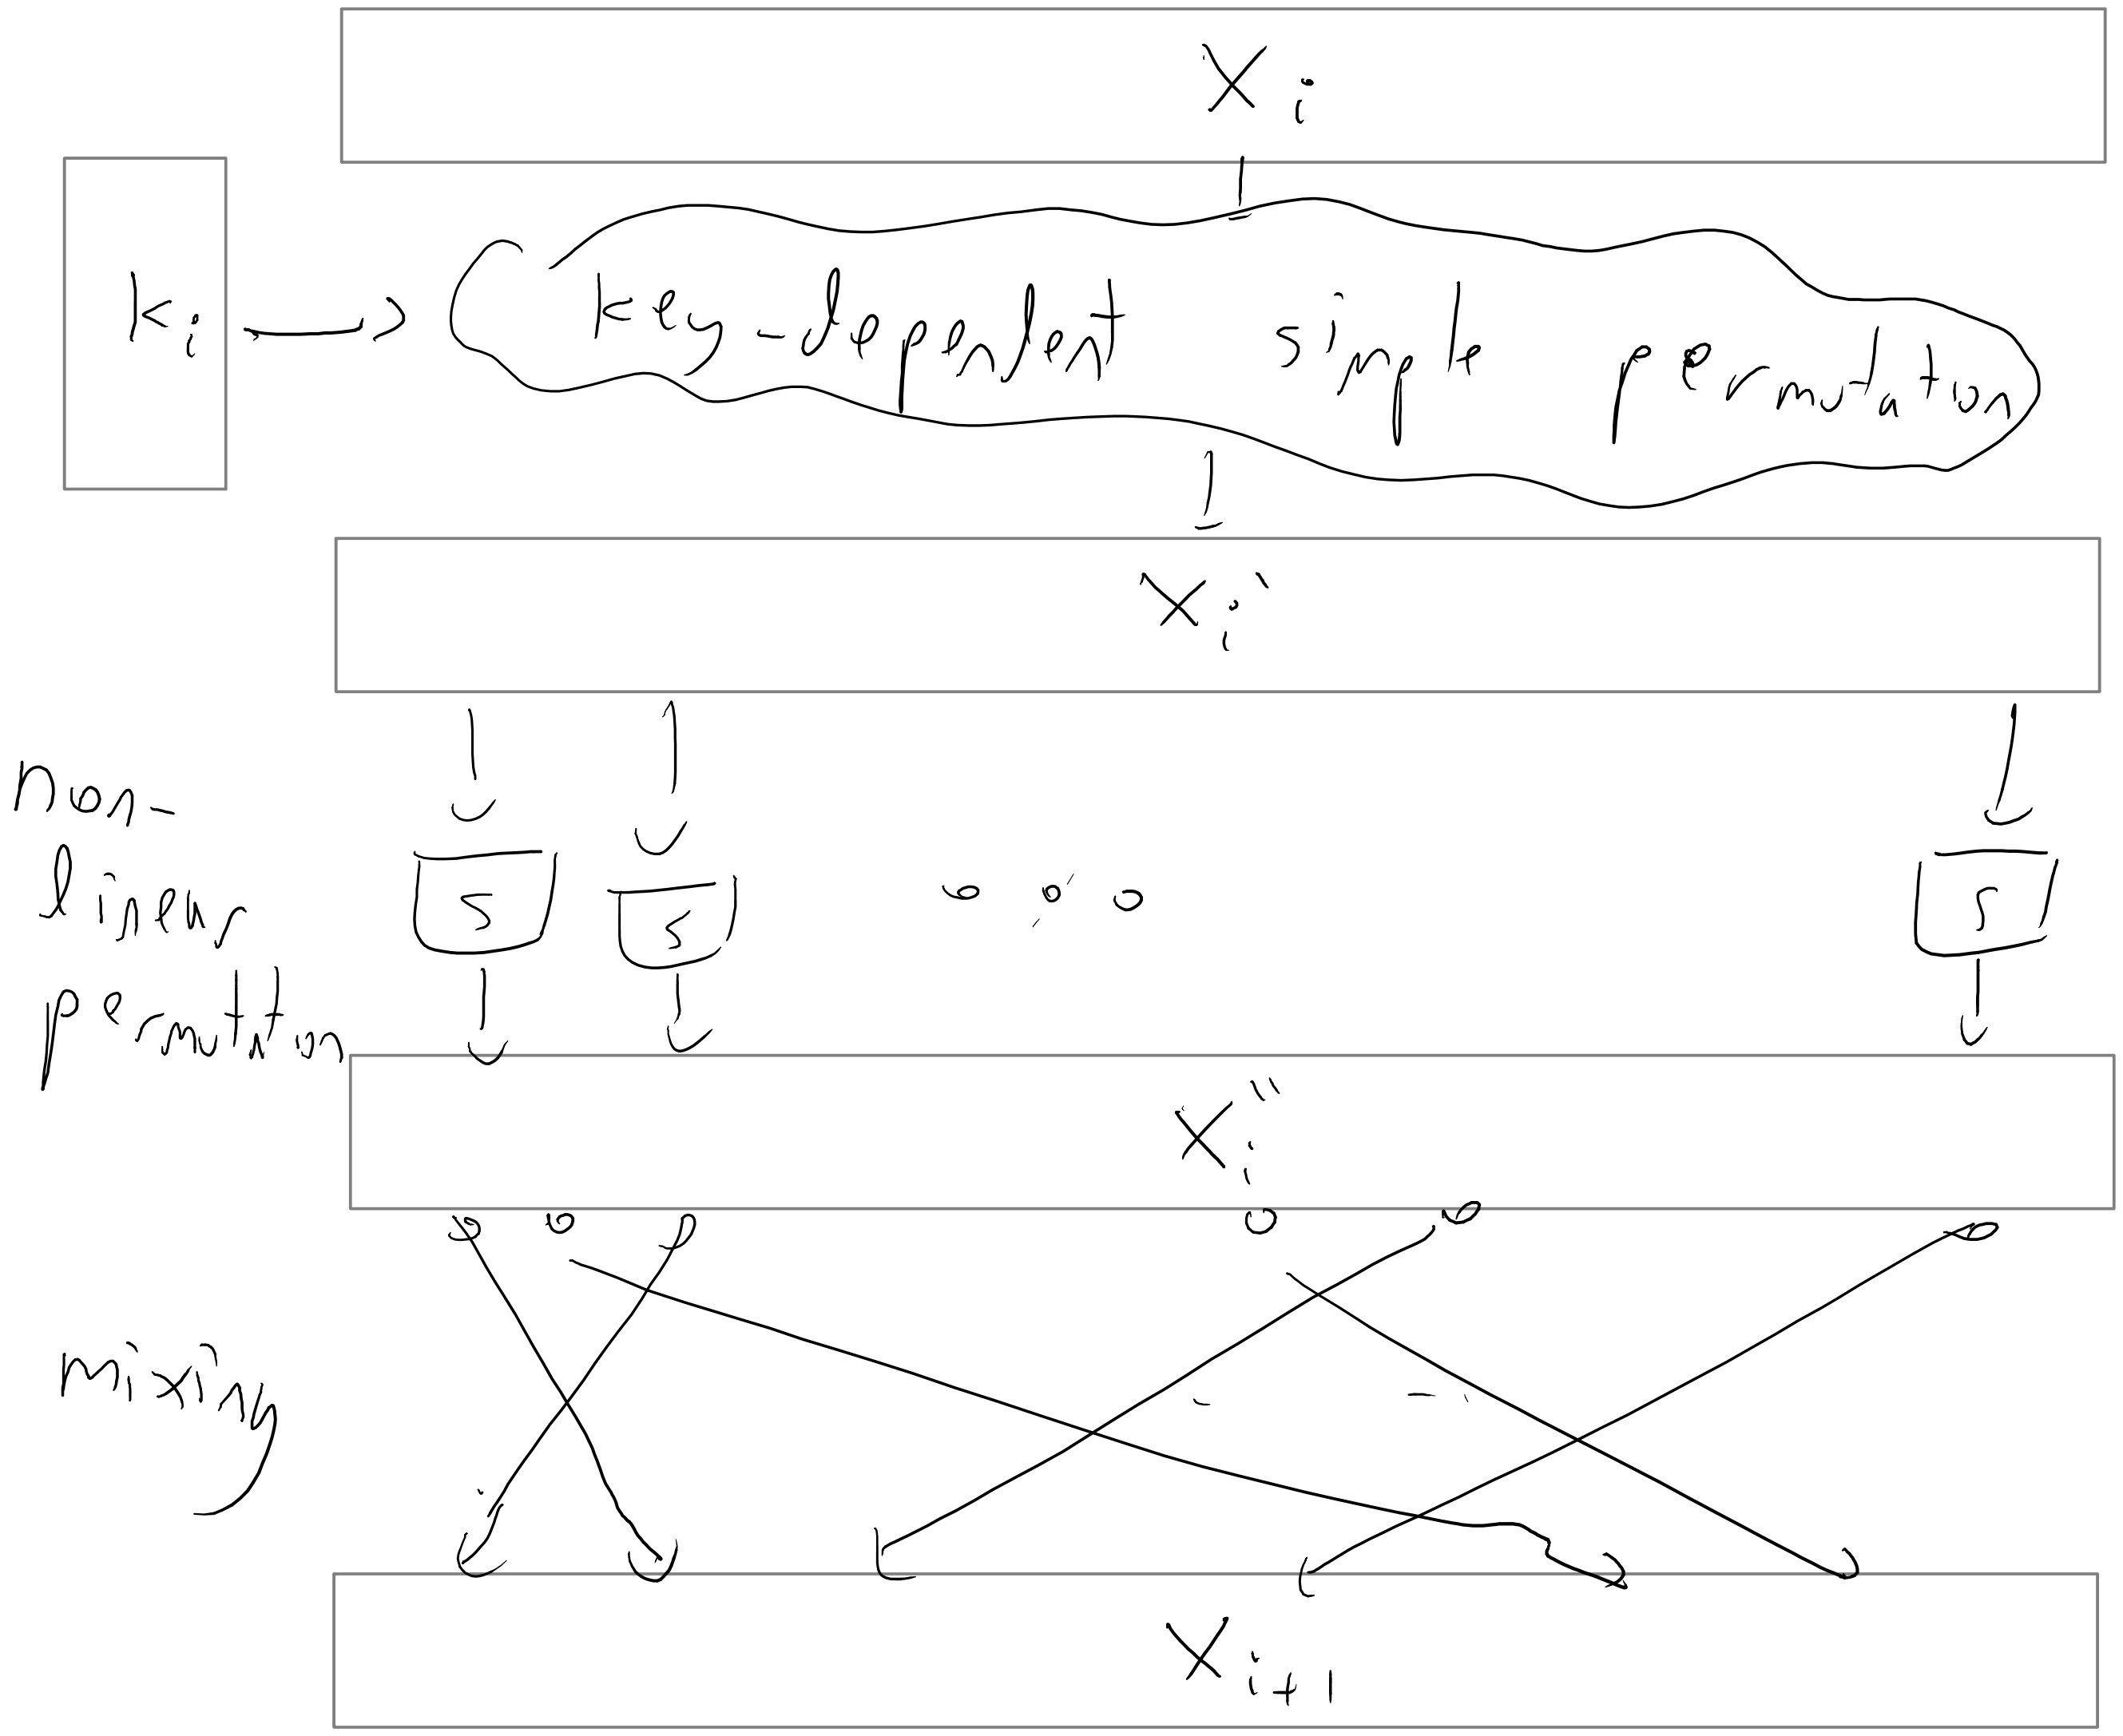
\includegraphics[width=\linewidth, height=1.5in, keepaspectratio]{../figure/block-cipher-round.jpg}
\caption{A typical round of a block cipher, \(k_i\) is the \(i^{th}\)
round key, \(x_i\) is the block before the \(i^{th}\) round and
\(x_{i+1}\) is the block at the end of this round.}
\label{blockcipherfig}
\end{marginfigure}

\section{Encryption modes}\label{5-Encryption-modes}

How do we use a block cipher to actually encrypt traffic? Well we could
use it as a PRF in the construction above, but in practice people use
other ways.\footnote{Partially this is because in the above construction
  we had to encode a plaintext of length \(n\) with a ciphertext of
  length \(2n\) meaning an overhead of 100 percent in the communication.}

The most natural approach would be that to encrypt a message \(m\), we
simply use \(p_s(m)\) where \(\{ p_s \}\) is the PRP/block cipher. This
is known as the \emph{electronic code book (ECB) mode} of a block cipher
(see \cref{ecbonefig}). Note that we can easily decrypt since we can
compute \(p_s^{-1}(m)\). If the PRP \(\{p_s\}\) only accepts inputs of a
fixed length \(\ell\), we can use ECB mode to encrypt a message \(m\)
whose length is a multiple of \(\ell\) by writing
\(m = (m_1, m_2, \ldots, m_t)\), where each block \(m_i\) has length
\(\ell\), and then encrypting each block \(m_i\) separately. The
ciphertext output by this encryption scheme is
\((p_s(m_1), \ldots, p_s(m_t))\). A major drawback of ECB mode is that
it is a \emph{deterministic} encryption scheme and hence cannot be CPA
secure. Moreover, this is actually a real problem of security on
realistic inputs (see \cref{ecbtwofig}), so ECB mode should never be
used.

\begin{marginfigure}
\centering
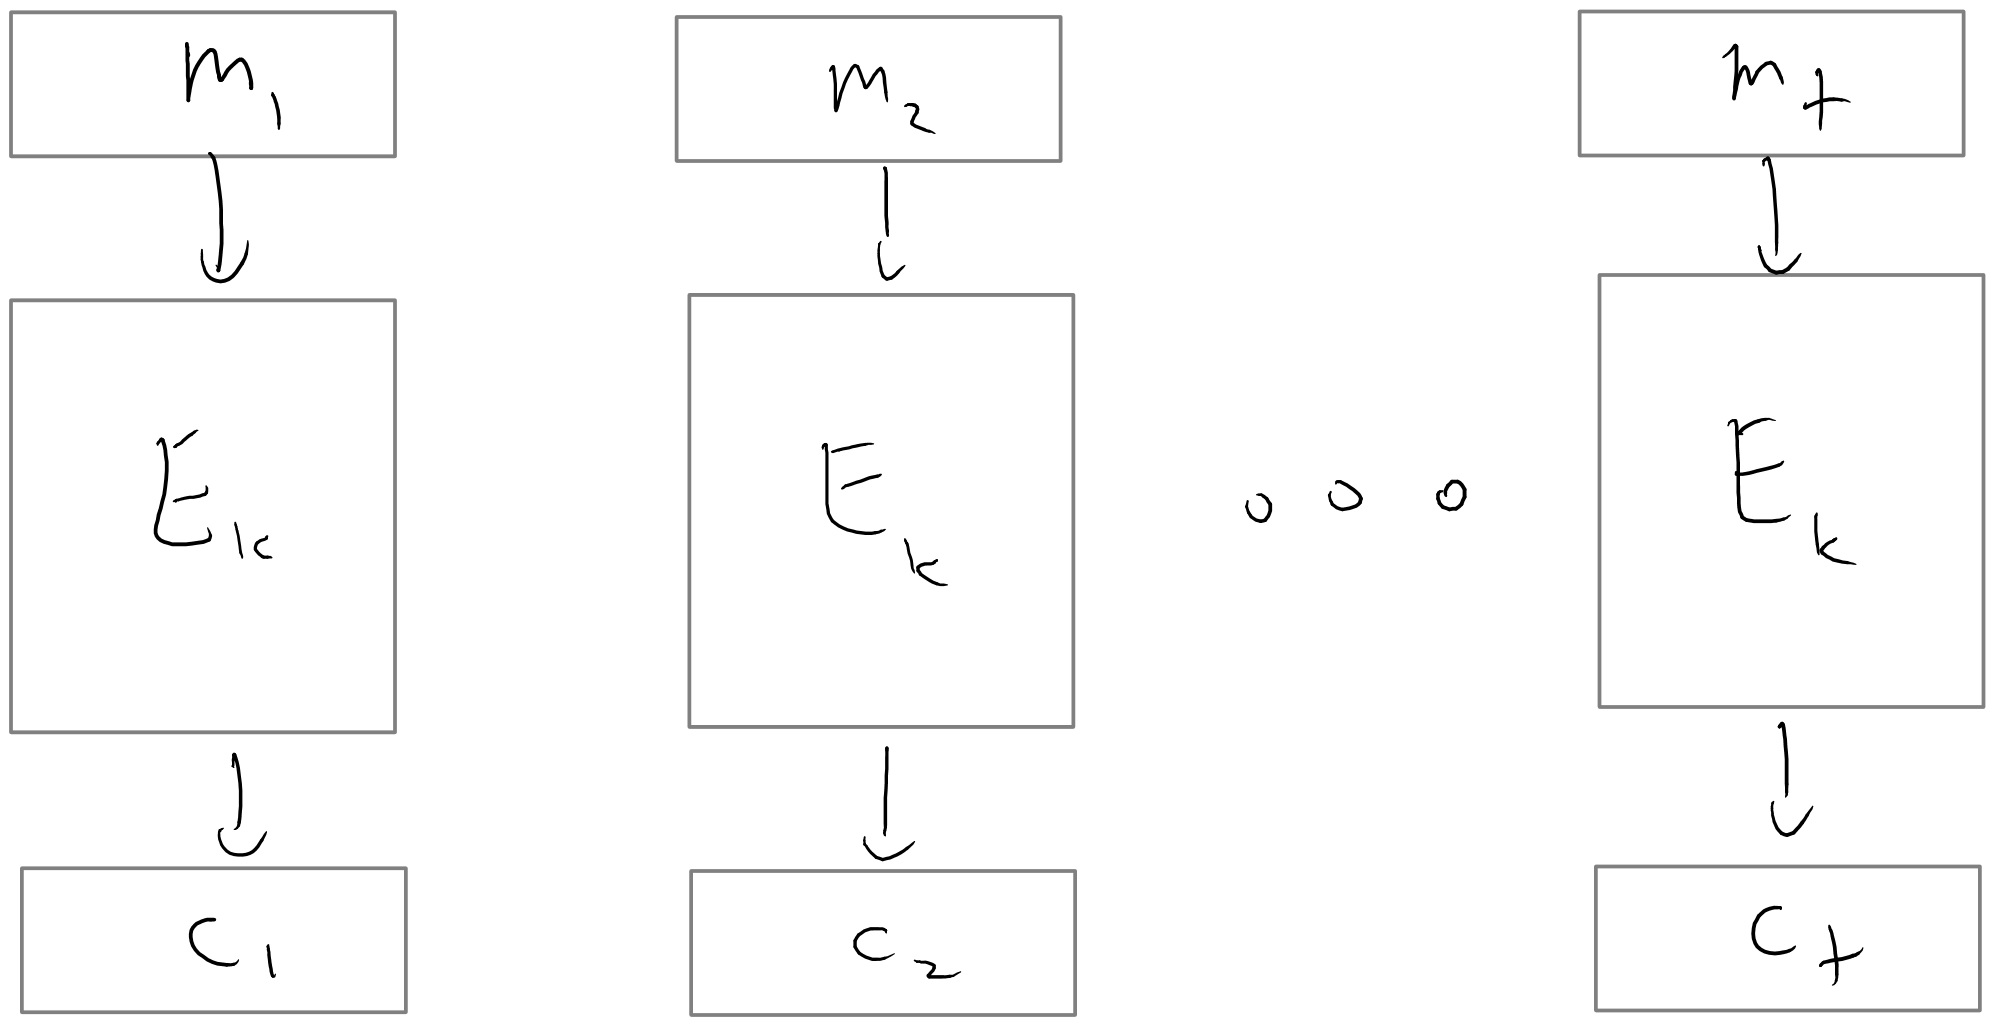
\includegraphics[width=\linewidth, height=1.5in, keepaspectratio]{../figure/ecb-mode.jpg}
\caption{In the Electronic Codebook (ECB) mode, every message is
encrypted deterministically and independently}
\label{ecbonefig}
\end{marginfigure}

\begin{marginfigure}
\centering
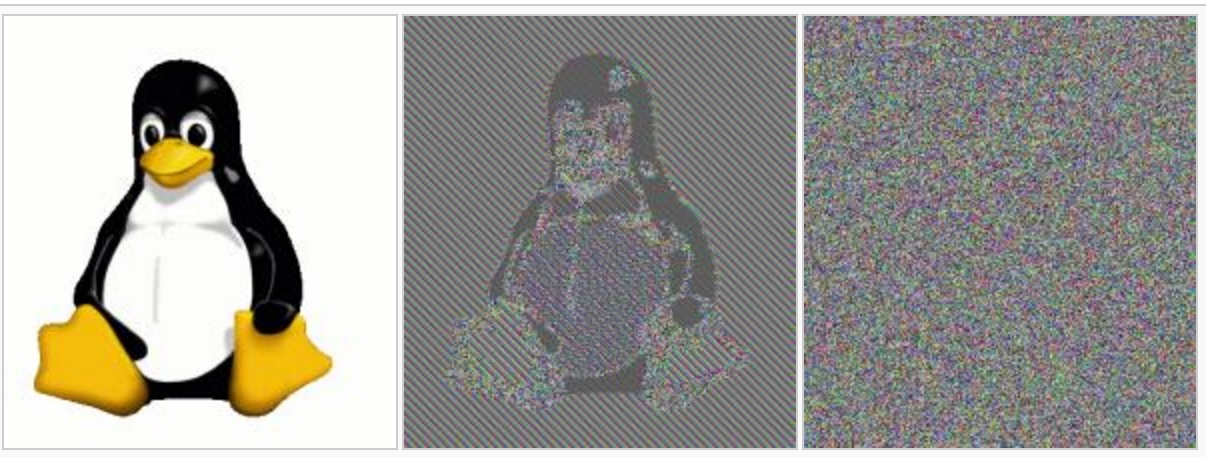
\includegraphics[width=\linewidth, height=1.5in, keepaspectratio]{../figure/ECB_prob.jpg}
\caption{An encryption of the Linux penguin (left image) using ECB mode
(middle image) vs CBC mode (right image). The ECB encryption is insecure
as it reveals much structure about the original image. Image taken from
Wikipedia.}
\label{ecbtwofig}
\end{marginfigure}

A more secure way to use a block cipher to encrypt is the \emph{cipher
block chaining (CBC) mode}. The idea of cipher block chaining is to
encrypt the blocks of a message \(m = (m_1, \ldots, m_t)\) sequentially.
To encrypt the first block \(m_1\), we XOR \(m_1\) with a random string
known as the \emph{initialization vector}, or
\(\ensuremath{\mathit{IV}}\), before applying the block cipher \(p_s\).
To encrypt one of the later blocks \(m_i\), where \(i > 1\), we XOR
\(m_i\) with the \emph{encryption} of \(m_{i-1}\) before applying the
block cipher \(p_s\). Formally, the ciphertext consists of the tuple
\((\ensuremath{\mathit{IV}}, c_1, \ldots, c_t)\), where
\(\ensuremath{\mathit{IV}}\) is chosen uniformly at random and
\(c_i = p_s(c_{i-1} \oplus m_i)\) for \(1 \le i \le t\) (we use the
convention that \(c_0 = \ensuremath{\mathit{IV}}\)). This encryption
process is depicted in \cref{cbcmodefig}. In order to decrypt
\((\ensuremath{\mathit{IV}}, c_1, \ldots, c_t)\), we simply calculate
\(m_i = p_s^{-1}(c_i) \oplus c_{i-1}\) for \(1 \le i \le t\). Note that
if we lose the block \(c_i\) to traffic in the CBC mode, then we are
unable to decrypt the next block \(c_{i+1}\), but we can recover from
that point onwards.

On the one hand, CBC mode is vastly superior to a simple electronic
codebook since CBC mode with a random \(\ensuremath{\mathit{IV}}\) is
CPA secure (proving this is an excellent exercise). On the other hand,
CBC mode suffers from the drawback that the encryption process cannot be
parallelized: the ciphertext block \(c_i\) \emph{must} be computed
before \(c_{i+1}\).

\begin{marginfigure}
\centering
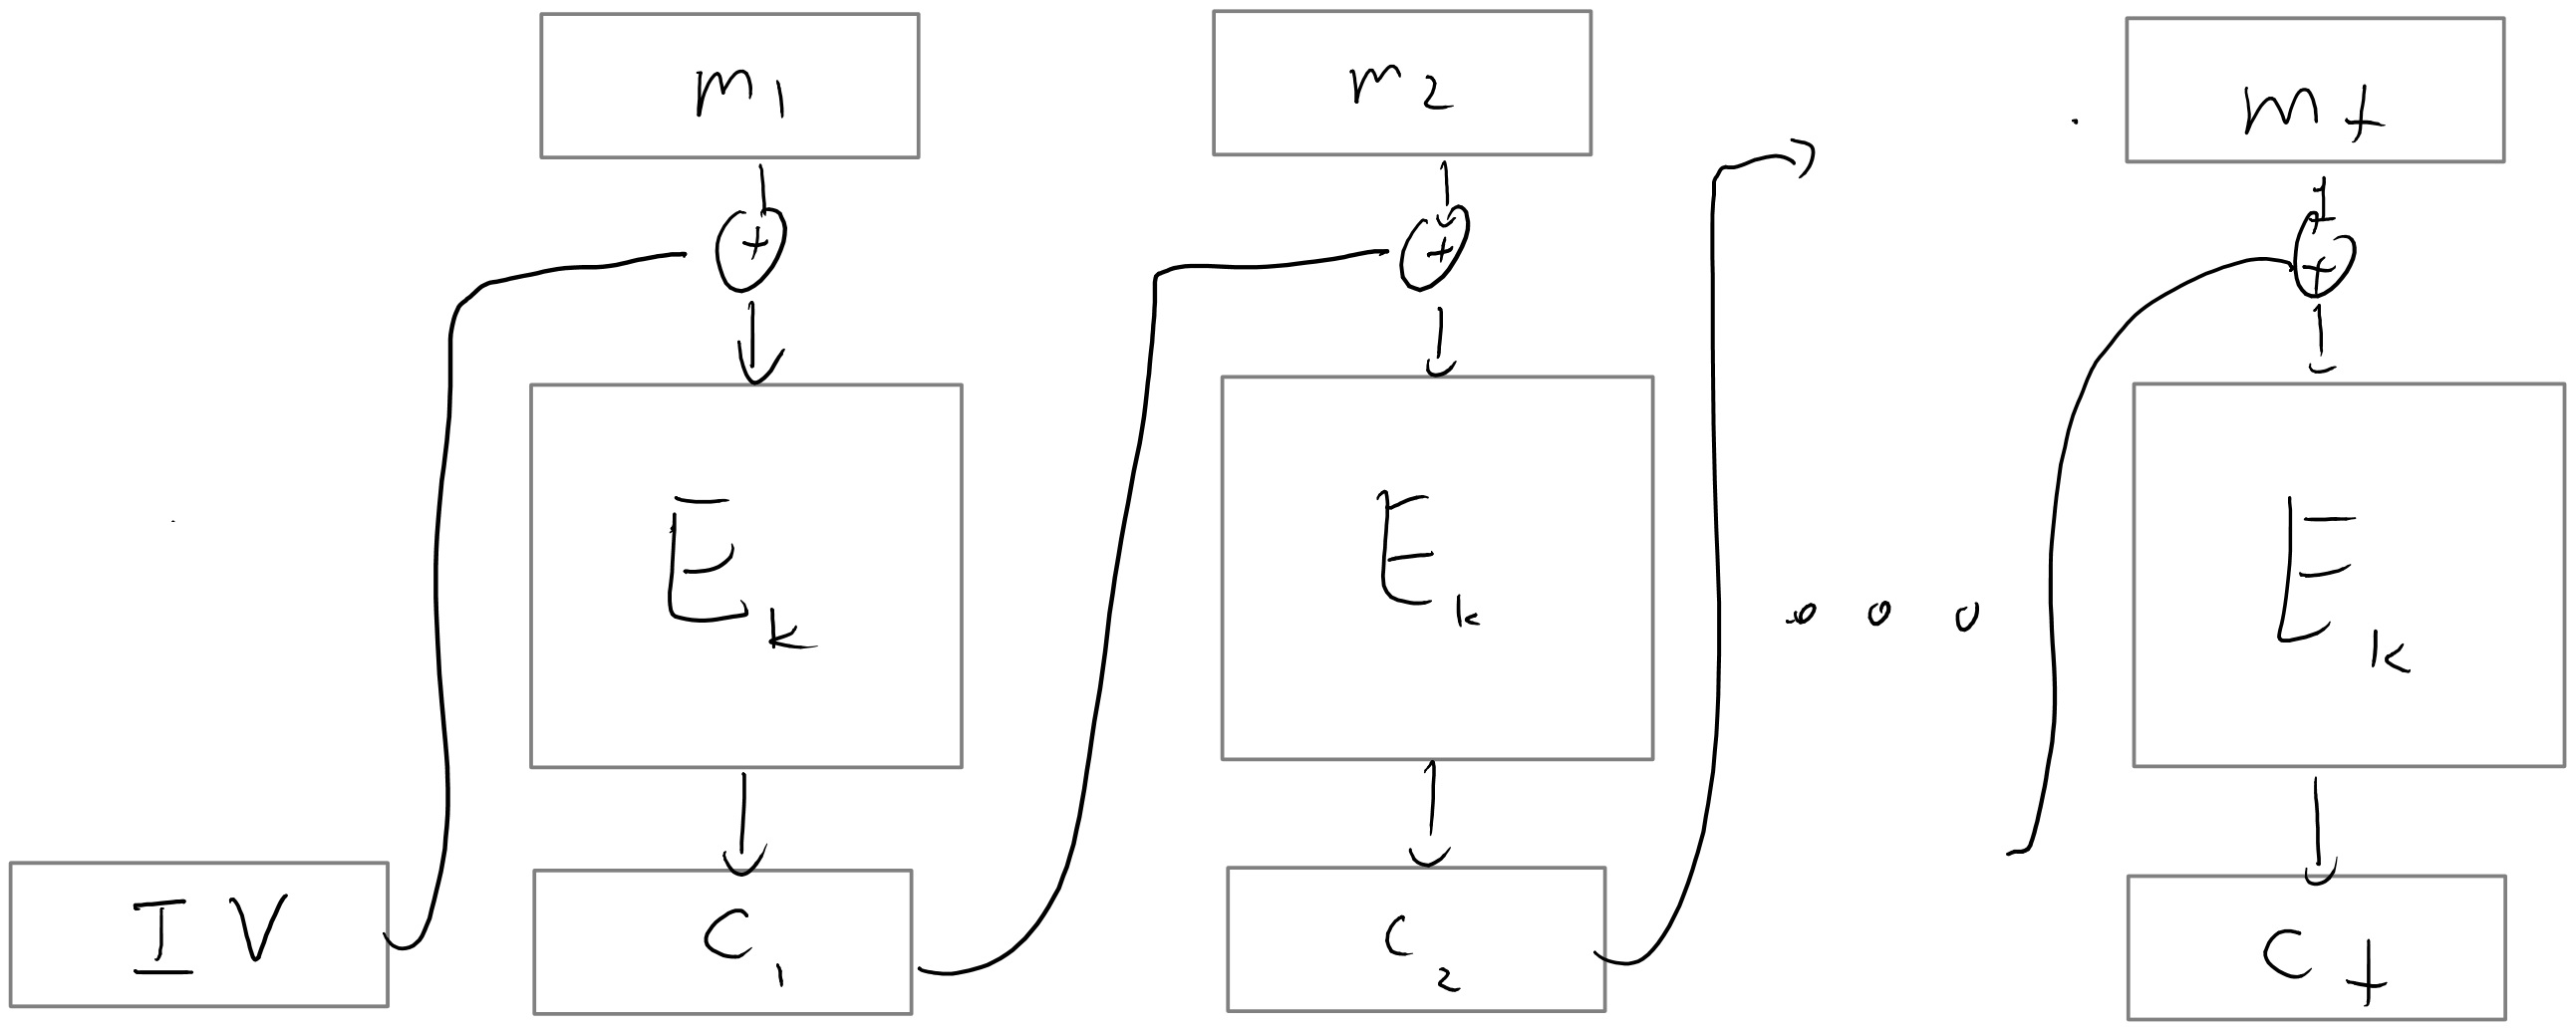
\includegraphics[width=\linewidth, height=1.5in, keepaspectratio]{../figure/cbc-mode.jpg}
\caption{In the Cypher-Block-Chaining (CBC) the encryption of the
previous message is XOR'ed into the current message prior to encrypting.
The first message is XOR'ed with an \emph{initialization vector} (IV)
that if chosen randomly, ensures CPA security.}
\label{cbcmodefig}
\end{marginfigure}

In the \emph{output feedback (OFB) mode} we first encrypt the all zero
string using CBC mode to get a sequence \((y_1,y_2,\ldots)\) of
pseudorandom outputs that we can use as a stream cipher. To transmit a
message \(m \in \{0,1\}^*\), we send the XOR of \(m\) with the bits
output by this stream cipher, along with the
\(\ensuremath{\mathit{IV}}\) used to generate the sequence. The receiver
can decrypt a ciphertext \((\ensuremath{\mathit{IV}}, c)\) by first
using \(\ensuremath{\mathit{IV}}\) to recover \((y_1, y_2, \ldots)\),
and then taking the XOR of \(c\) with the appropriate number of bits
from this sequence. Like CBC mode, OFB mode is CPA secure when
\(\ensuremath{\mathit{IV}}\) is chosen at random. Some advantages of OFB
mode over CBC mode include the ability for the sender to precompute the
sequence \((y_1, y_2, \ldots)\) well before the message to be encrypted
is known, as well as the fact that the underlying function \(p_s\) used
to generate \((y_1, y_2, \ldots)\) only needs to be a PRF (not
necessarily a PRP).

Perhaps the simplest mode of operation is \emph{counter (CTR) mode}
where we convert a block cipher to a stream cipher by using the stream
\(p_s(\ensuremath{\mathit{IV}}),p_s(\ensuremath{\mathit{IV}}+1),p_s(\ensuremath{\mathit{IV}}+2),\ldots\)
where \(\ensuremath{\mathit{IV}}\) is a random string in \(\{0,1\}^n\)
which we identify with \([2^n]\) (and perform addition modulo \(2^n\)).
That is, to encrypt a message \(m = (m_1, \ldots, m_t)\), we choose
\(\ensuremath{\mathit{IV}}\) at random, and output
\((\ensuremath{\mathit{IV}}, c_1, \ldots, c_t)\), where
\(c_i = p_s(\ensuremath{\mathit{IV}} + i) \oplus m_i\) for
\(1 \le i \le t\). Decryption is performed similarly. For a modern block
cipher, CTR mode is no less secure than CBC or OFB, and in fact offers
several advantages. For example, CTR mode can easily encrypt and decrypt
blocks in parallel, unlike CBC mode. In addition, CTR mode only needs to
evaluate \(p_s\) once to decrypt any single block of the ciphertext,
unlike OFB mode.

A fairly comprehensive study of the different modes of block ciphers is
in \href{http://web.cs.ucdavis.edu/~rogaway/papers/modes.pdf}{this
document by Rogaway}. His conclusion is that if we simply consider CPA
security (as opposed to the stronger notions of \emph{chosen ciphertext
security} we'll see in the next lecture) then counter mode is the best
choice, but CBC, OFB and CFB are widely implemented due to legacy
reasons. ECB should not be used (except as a building block as part of a
construction achieving stronger security).

\section{Optional, Aside: Broadcast
Encryption}\label{5-Optional-Aside-Broadca}

At the beginning of this chapter, we saw the proof of \cref{prfthm},
which states that the PRG Conjecture implies the existence of a secure
PRF collection. At the heart of this proof was a rather clever
construction based on a binary tree. As it turns out, similar tree
constructions have been used time and again to solve many other problems
in cryptography. In this section, we will discuss just one such
application of these tree constructions, namely \emph{broadcast
encryption}.

Let's put ourselves in the shoes of Hollywood executives facing the
following problem: we've just released a new movie for sale (in the form
of a download or a Blu-ray disc), and we'd like to prevent it from being
pirated. On the one hand, consumers who've purchased a copy of the movie
should be able to watch it on certain approved, standalone devices such
as TVs and Blu-ray players without needing an external internet
connection. On the other hand, to minimize the risk of piracy, these
consumers should \emph{not} have access to the movie data itself.

One way to protect the movie data, which we model as a string \(x\), is
to provide consumers with a secure encryption \(E_k(x)\) of the data.
Although the secret key \(k\) used to encrypt the data is hidden from
consumers, it is provided to device manufacturers so that they can embed
it in their TVs and Blu-ray players in some secure, tamper-resistant
manner. As long as the key \(k\) is never leaked to the public, this
system ensures that only approved devices can decrypt and play a
consumer's copy of the movie. For this reason, we will sometimes refer
to \(k\) as the \emph{device key}. This setup is depicted in
\cref{brdcastencfig}.

\begin{figure}
\centering
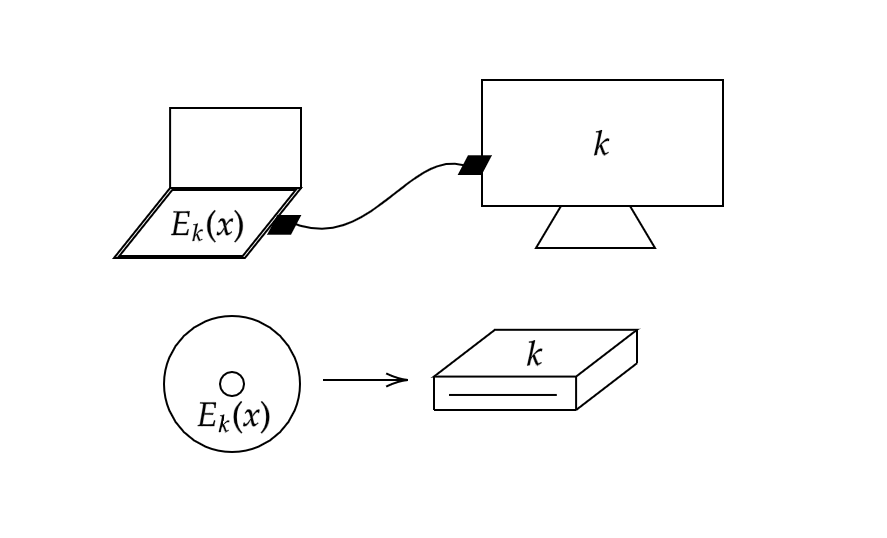
\includegraphics[width=\textwidth, height=0.25\paperheight, keepaspectratio]{../figure/brdcastencfig.png}
\caption{The problem setup for broadcast encryption.}
\label{brdcastencfig}
\end{figure}

Unfortunately, if we were to implement this scheme exactly as written,
it would almost certainly be broken in a matter of days. After all, as
soon as even a single device is hacked, the device key \(k\) would be
revealed. This would allow the public to access our movie's data, as
well as the data for \emph{all future movies} we release for these
devices! This latter consequence is one that we would certainly want to
avoid, and doing so requires the notion of distinct, \emph{revocable}
keys:

\hypertarget{broadcastdef}{}
\begin{definition}[Broadcast Encryption Scheme] \label[definition]{broadcastdef}

For our purposes, a \emph{broadcast encryption scheme} consists of:

\begin{itemize}
\item
  A set of \(m\) distinct devices (or device manufacturers), each of
  which has access to one of the \(n\)-bit device keys
  \(k_1, \ldots, k_m\).
\item
  A decryption algorithm \(D\) that receives as input a ciphertext \(y\)
  and a key \(k_i\).
\item
  An encryption algorithm \(E\) that receives as input a plaintext
  \(x\), a key \(k_{master}\), and a \emph{revocation set}
  \(R \subseteq [m]\) of devices (or device manufacturers) that are no
  longer to be trusted.
\end{itemize}

\end{definition}

Intuitively, a broadcast encryption scheme is secure if \(D_{k_i}\) can
successfully recover \(x\) from \(E_{k_{master}, R}(x)\) whenever
\(i \notin R\), but fails to do so whenever \(i \in R\). In our example
of movie piracy, such an encryption scheme would allow us to
\emph{revoke} certain device keys \(k_i\) when we find out that they
have been leaked. To revoke a key \(k_i\), we would simply include
\(i \in R\) when encrypting all future movies. Doing so prevents \(k_i\)
from being used to decrypt these movies. Crucially, revoking the key
\(k_i\) of the hacked device \(i\) doesn't prevent a secure device
\(j \neq i\) from continuing to perform decryption on future movie
releases; this is exactly what we want in our system.

For the sake of brevity, we will \emph{not} provide a formal definition
of security for broadcast encryption schemes, although this can and has
been done. Instead, in the remainder of this section, we will describe a
couple examples of broadcast encryption schemes, one of which makes
clever use of a tree construction, as promised.

The simplest construction of a broadcast encryption scheme involves
letting \(k_{master} = (k_1, \ldots, k_m)\) be the collection of all
device keys and letting \(E_{k_{master}, R}(x)\) be the concatenation
over all \(i \notin R\) of a secure encryption \(E_{k_i}(x)\). Device
\(i\) performs decryption by looking up the relevant substring
\(E_{k_i}(x)\) of the ciphertext and decrypting it with \(k_i\).
Intuitively, with this scheme, if \(x\) represents our movie data and
there are \(m \approx\) one million devices, then
\(E_{k_{master}, R}(x)\) is just an encryption of one million copies of
the movie (one for each device key). Revoking the key \(k_i\) amounts to
only encrypting \(999,999\) copies of all future movies, so that device
\(i\) can no longer perform decryption.

Clearly, this simple solution to the broadcast encryption problem has
two serious inefficiencies: the length of the master key is \(O(nm)\),
and the length of each encryption is \(O(|x|m)\). One way to address the
former problem is to use a \emph{key derivation function}. That is, we
can shorten the master key by choosing a fixed PRF collection
\(\{f_k\}\), and calculating each device key \(k_i\) by the rule
\(k_i = f_{k_{master}}(i)\). The latter problem can be addressed using a
technique known as \emph{hybrid encryption}. In hybrid encryption, we
encrypt \(x\) by first choosing an ephemeral key
\(\hat k \leftarrow_R \{0,1\}^n\), encrypting \(\hat k\) using each
device key \(k_i\) where \(i \notin R\), and then outputting the
concatenation of these strings \(E_{k_i}(\hat k)\), along with a
\emph{single} encryption \(E_{\hat k}(x)\) of the movie using the
ephermal key. Incorporating these two optimizations reduces the length
of \(k_{master}\) to \(O(n)\) and the length of each encryption to
\(O(nm + |x|)\).

\begin{figure}
\centering
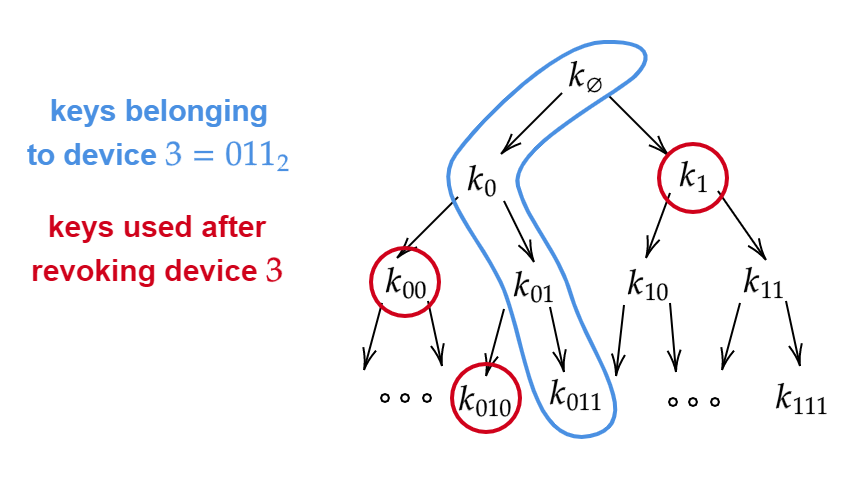
\includegraphics[width=\textwidth, height=0.25\paperheight, keepaspectratio]{../figure/brdcasttreefig.png}
\caption{A tree based construction of broadcast encryption with
revocable keys.}
\label{brdcasttreefig}
\end{figure}

It turns out that we can construct a broadcast encryption scheme with
even shorter ciphertexts by considering a \emph{tree of keys} (see
\cref{brdcasttreefig}). The root of this tree is labeled
\(k_{\varnothing}\), its children are \(k_0\) and \(k_1\), their
children are \(k_{00}, k_{01}, k_{10}, k_{11}\), and so on. The depth of
the tree is \(\log_2 m\), and the value of each key in the tree is
decided uniformly at random, or by applying a key derivation function to
a string \(k_{master}\). Each device \(i\) receives \emph{all} the keys
on the path from the root to the \(i\)th leaf. For example, if \(m=8\),
then device \(011\) receives the keys
\(k_{\varnothing}, k_0, k_{01}, k_{011}\).

To encrypt a message \(x\), we carry out the following procedure:
initially, when no keys have been revoked, we encrypt \(x\) using an
ephermal key \(\hat k\) (as described above) and encrypt \(\hat k\) with
a single device key \(k_\varnothing\). This is sufficient since all
devices have access to \(k_\varnothing\). In order to add a hacked
device \(i\) to the revocation set, we discard all \(\log_2 m\) keys
belonging to device \(i\), which comprise a root-to-leaf path in the
tree. Instead of using these keys, we will make sure to encrypt all
future \(\hat k\)'s using the \emph{siblings} of the vertices along this
path. Doing so ensures that (1) device \(i\) can no longer decrypt
secure content and (2) every device \(j \neq i\) can \emph{continue} to
decrypt content using at least one of the keys along the path from the
root to the \(j\)th leaf. With this scheme, the total length of a
ciphertext is only \(O(n|R| \log_2 m + |x|)\) bits, where \(|R|\) is the
number of devices revoked so far. When \(|R|\) is small, this bound is
\emph{much} better than what we previously achieved without a tree-based
construction.

\section{Reading comprehension
exercises}\label{5-Reading-comprehension-}

I recommend students do the following exercises after reading the
lecture. They do not cover all material, but can be a good way to check
your understanding.

\begin{exercise} \label[exercise]{5-Let-ED-be-the-encrypti}

Let \((E,D)\) be the encryption scheme that we saw in Lecture 2 where
\(E_k(m)=G(k)\oplus m\) where \(G(\cdot)\) is a pseudorandom generator.
Is this scheme CPA secure?

\begin{enumerate}
\def\labelenumi{\alph{enumi}.}
\tightlist
\item
  No it is never CPA secure.
\item
  It is always CPA secure.
\item
  It is sometimes CPA secure and sometimes not, depending on the
  properties of the PRG \(G\)
\end{enumerate}

\end{exercise}

\begin{exercise} \label[exercise]{5-Consider-the-proof-con}

Consider the proof constructing PRFs from PRGs. Up to an order of
magnitude, how many invocations of the underlying pseudorandom generator
does the pseudorandom function collection make when queried on an input
\(i\in \{0,1\}^n\)?

\begin{enumerate}
\def\labelenumi{\alph{enumi}.}
\tightlist
\item
  \(n\)
\item
  \(n^2\)
\item
  \(1\)
\item
  \(2^n\)
\end{enumerate}

\end{exercise}

\begin{exercise} \label[exercise]{5-In-the-following-we-id}

In the following we identify a block cipher with a pseudorandom
permutation (PRP) collection. Which of these statements is true:

\begin{enumerate}
\def\labelenumi{\alph{enumi}.}
\tightlist
\item
  Every PRP collection is also a PRF collection
\item
  Every PRF collection is also a PRP collection
\item
  If \(\{ f_s \}\) is a PRP collection then the encryption scheme
  \(E_s(m)=f_s(m)\) is a CPA secure encryption scheme.
\item
  If \(\{ f_s \}\) is a PRF collection then the encryption scheme
  \(E_s(m)=f_s(m)\) is a CPA secure encryption scheme.
\end{enumerate}

\end{exercise}
